\section{Introduction}
\label{ap:Closure_problem}

The equations governing the closure problem are often derived based on physical principles or intuitive reasoning.
For example, to determine the drag force term in the averaged momentum equation, in the dilute limit, the problem of a translating sphere in an unbounded flow with background velocity $\textbf{u}^\infty$ is commonly considered \citep{stone2001inertial,raja2010inertial,guazzelli2011}.
"background velocity" refers to the undisturbed flow at the particle location as if the particle were not present.


However, in the context of averaged equations, one might wonder: does $\textbf{u}^\infty$ correspond to the averaged fluid velocity $\textbf{u}_f$ (as used in \citet{jackson1997locally,zhang1997momentum}), the bulk velocity $\textbf{u}$ \citep{kim1985modelling}, or the Favre-averaged velocity $\textbf{u}_m$?
In other words, how can we relate the ensemble-averaged properties of the "hybrid" or "two-fluid" model to the closure terms?

As demonstrated, this question introduces the need for a rigorous statistical derivation of the closure problem.

The closure terms in the ``Hybrid'' model are the results of the ensemble average operator $\avg{\ldots}$. 
In all rigor, we cannot compute theoretically such an average since it necessitates knowing the distribution $P(\FF)$ and the exact expression of the local terms indicated by the notation $(\ldots)^0$. 
In the same spirit as in \citet{buyevich1979flow,lhuillier1992ensemble,batchelor1972sedimentation,hinch1977averaged} and \citet{zhang1994averaged} we demonstrate here that it is therefore necessary to reformulate the closure term to remove the ensemble average procedure. 
We demonstrated in \ref{ap:Closure_problem} that any ensemble-averaged quantities can be reformulated as an integral of what we call \textit{conditionally-averaged quantities}. 
The expressions obtained are  consistent with \citet{batchelor1972sedimentation,hinch1977averaged} and \citet[Appendix A]{zhang1994averaged} which also proposed conditional averages, but somewhat more general because our methodology applies to any closure term of the ``Hybrid model''. 
In a second step, we demonstrate how to derive what we call the \textit{conditionally-averaged equations} that are needed to obtain the \textit{conditionally-averaged quantities}. 

In the limit of Stokes flows \citet{hinch1977averaged} were the first authors to introduce this methodology.
He used the \textit{conditionally-averaged equations} to re-demonstrate, as a proof of concept, the bulk stress of a suspension of solid spheres at $\mathcal{O}(\phi^2)$ and the sedimentation velocity of the dispersed phase at $\mathcal{O}(\phi^2)$. 
In \citet{kim1985modelling} they use the \textit{conditionally-averaged equations} to consider the effect of finite volume fraction on the drag force closure term, in fixed beds of spherical solid spheres, their analysis holds for arbitrary volume fraction $\phi$. 

Again our derivation is directly inspired by the cited author, but the approach is generalized by considering fluid inclusion and an inertial regime. 
For instance, in the dilute regime, the \textit{conditionally-averaged equations} correspond to the problem of the disturbance field generated by an isolated translating droplet. 
The real interest behind this demonstration is that it is kept general and offers many possibilities for model extension.
 




% In \ref{sec:reformulation} and \ref{sec:the_disturbance_eq} we discuss the general approach to derive the closure problem
%%%%%%%%%%%%%%%%%%% A mettre dans lautre chap
% , while in \ref{sec:application} we derive the closures terms of the momentum and energy equations. 
% Since the derivation of the closure terms can be understood through physical arguments, readers who are less interested in the rigorous mathematical formulation of the closure problem, which can be quite involved, may skip directly to \ref{sec:application}.


\section{Reformulation of the closure terms}
\label{sec:reformulation}

% We aim to compute our closures within the dilute Stokes flow regime for spherical particles of radius $a$. 
% In this regime we expect that the closure terms will only be determined by the center of mass velocity of the droplets ($\textbf{u}_p$), their position in space, and the macroscopic properties of the continuous phase ($\textbf{u}_f, \grad \textbf{u}_f \ldots$). 
% Indeed, as we will demonstrate in the following section, only these properties define the boundaries of the \textit{single-particle} conditionally-averaged equations, and are therefore sufficient to achieve closure of the problem  in the Stokes flow regime. 

In the following, we express our closures in terms of averaged quantities, conditioned on the position of the center of mass of a \textit{test-particle} and its center of mass velocity. 
Note that for shape-dependent closure terms it would also be necessary to obtain the \textit{shape-conditioned} averaged fields, but this is out of the scope of this work.
Similarly, to account for the contribution of droplet acceleration to the closure terms (such as the added mass effect), it would be necessary to consider the \textit{center-of-mass-acceleration-conditioned} averaged fields.
However, this lies beyond the scope of the present work.
  
\subsection{Interfacial terms}

In the equations presented in \ref{sec:application} certain closures, such as surface stresses and surface heat fluxes, are expressed in the form of particle-averaged surface integrals. 
Here, we focus on reformulating these terms in terms of \textit{single-particle} conditionally-averaged quantities, which will be defined in the subsequent sections.

As the procedure is similar for all surface particle-averaged terms, let us take the example of the exchange of momentum term appearing in the continuous and dispersed phase averaged momentum equations (\ref{eq:dt_hybrid_rhou_f} and \ref{eq:dt_hybrid_up}). 
From the definition of the particle average we write,
\begin{align}
    \pSavg{\bm\sigma_f^0\cdot\textbf{n}}[\textbf{x},t]
    &= \avg{ \sum_{\alpha=1}^N \delta(\textbf{x}-\textbf{x}_\alpha[t; \FF])
    \int_{\Gamma_\alpha(t,\FF)}
    (\bm\sigma_f^0\cdot\textbf{n})[\textbf{y},t;\FF]
    d\Gamma[\textbf{y}] }
    \label{eq:first_step_reallay}
\end{align}
By writing this integral explicitly, we emphasize that the particle-averaged quantity (left-hand side of \ref{eq:first_step_reallay}) is evaluated at the point \textbf{x}, while the parameter $\textbf{y}$ is used for the integration over the particle's surface.
Recall that $\Gamma_\alpha$ refers to the surface of the droplet $\alpha$ and $\textbf{x}_\alpha$ to the position of the center of mass of that same droplet $\alpha$. 
Thus, the notation $(\bm\sigma_f^0\cdot\textbf{n})[\textbf{y},t;\FF]$ means that we evaluate the local stress as well as the local normal $\textbf{n}$ to the particle, at \textbf{y}. 
We now enlarge the domain of integration from $\Gamma_\alpha$ (the surface of the particle $\alpha$) to $\mathbb{R}^3$ with the introduction of the interface indicator function of the particle $\alpha$, namely $\delta(|\textbf{y} - \textbf{x}_\alpha[t,\FF]| - a)$\footnote{Indeed, for spherical particles, we can define the interface indicator function of a single particle using the definition $\delta_\Gamma = \delta(|\textbf{y} - \textbf{x}_\alpha[t,\FF]| - a)$.}. 
It reads,
\begin{multline}
    \pSavg{\bm\sigma_f^0\cdot\textbf{n}}[\textbf{x},t]
    = \\
    \int_{\mathbb{R}^3}
    \avg{
     \sum_{\alpha=1}^N 
     \delta(\textbf{x}-\textbf{x}_\alpha[t \FF])
    \delta(|\textbf{y} - \textbf{x}_{\alpha}[t;\FF]|-a)
    (\bm\sigma_f^0\cdot\textbf{n})[\textbf{y},t;\FF]
    }
    d\textbf{y}. 
    \label{eq:first_step_drag}
\end{multline} 
Since the domain of integration $\mathbb{R}^3$ is now independent of $\FF$, we may substitute the integral and ensemble average operator. 

As mentioned above, we assume that the closure terms are entirely determined by the center of mass velocity of the particles and their position in space. 
Therefore, to include the condition on the particle velocity we introduce the relation 
\begin{equation}
    \int_{\mathbb{R}^3} \delta(\textbf{w} - \textbf{u}_\alpha[\FF,t]) d\textbf{w} = 1,
    \label{eq:Pw_normed}
\end{equation}
where $\textbf{w}$ is the test-particle center of mass velocity in the Eulerian space and $\textbf{u}_\alpha$ is the center of mass velocity within the Lagrangian framework. 
Injecting \ref{eq:Pw_normed} into \ref{eq:first_step_drag} one obtains, 
\begin{multline}
    \pSavg{\bm\sigma_f^0\cdot\textbf{n}}[\textbf{x},t]
    = \\
    \int_{\mathbb{R}^3}
    \int_{\mathbb{R}^3}
    \avg{
     \sum_{\alpha=1}^N 
     \delta(\textbf{x}-\textbf{x}_\alpha[t \FF])
     \delta(\textbf{w} - \textbf{u}_\alpha[\FF,t])
    \delta(|\textbf{y} - \textbf{x}_{\alpha}[t;\FF]|-a)
    (\bm\sigma_f^0\cdot\textbf{n})[\textbf{y},t;\FF]
    }
    d\textbf{y}
    d\textbf{w}. 
    \label{eq:second_step_drag}
\end{multline}
The quantity with the ensemble average operator now represents the average of the local stress $(\bm\sigma_f^0\cdot\textbf{n})[\textbf{y},t;\FF]$ on every configuration where the interface of a droplet is present at \textbf{y} with its center of mass at \textbf{x} and with a center of mass velocity \textbf{w}.


Moreover, since the expression within the ensemble average in \ref{eq:first_step_drag} is identically zero when, $\textbf{x}_\alpha \neq \textbf{x}$, we may replace the interface indicator function such that 
\begin{equation}
    \delta(\textbf{x}-\textbf{x}_\alpha[t,\FF])\delta(|\textbf{y} - \textbf{x}_{\alpha}[t,\FF]|-a) = \delta(\textbf{x}-\textbf{x}_\alpha[t,\FF])\delta(|\textbf{y} - \textbf{x}|-a). 
    \label{eq:from_R3_to_S}
\end{equation}
Since the function $\delta(|\textbf{y} - \textbf{x}|-a)$ is not dependent on $\FF$ it can be taken out of the ensemble average operator, hence reducing the domain of integration from $\mathbb{R}^3$ to $|\textbf{y}-\textbf{x}| = a$ in \ref{eq:first_step_drag}. 
\footnote{For deformable or non-spherical particles, this function may take a more complicated form, since the interface of a deformable or anisotropic particle is not entirely determinate by its center of mass position. 
It is clear that if the position of the interface is conditioned by the exact shape of the interface, then we can always express the interface indicator function as $\delta(f(\textbf{x}))$ where $f$ is a distance function of the shape that may depend on the particle's orientation (for anisotropic particles) or aspect ratio (for slightly deformable ones). 
Anyhow, this approach is generalizable to other kinds of particles, but in this work, we consider only spherical droplets. 
Note that for spheroidal particles as in \ref{chap:deformable} we may write $\delta_{\alpha\Gamma} = \delta((\textbf{y} - \textbf{x}_\alpha[t,\FF])\cdot (\bm\chi_\alpha+\bm\delta)\cdot(\textbf{y} - \textbf{x}_\alpha[t,\FF]) - a^2)$ where we have used the notation of \ref{chap:deformable}
}

Injecting \ref{eq:from_R3_to_S} into \ref{eq:second_step_drag} and using the last remark leads us to the relation 
\begin{equation}
    \pSavg{\bm\sigma_f^0\cdot\textbf{n}}[\textbf{x},t]
    =
    \int_{\mathbb{R}^3}
    P_1[\textbf{x},\textbf{w},t]
    \int_{|\textbf{x}-\textbf{y}|=a}
    (\bm\sigma_f^1 \cdot \textbf{n})[\textbf{y},\textbf{x},\textbf{w},t]
    d\textbf{y}
    d\textbf{w}
    \label{eq:conditionally_averaged}
\end{equation}
where we introduced the definitions, 
\begin{align}
    \bm\sigma^1_f[\textbf{y},\textbf{x},\textbf{w},t]
    % \phi_I^1[\textbf{y}|\textbf{x},\textbf{w},t] 
    % P_1[\textbf{x},\textbf{w},t]
    &= 
    \frac{1}{P_1}
    \avg{
    \sum_\alpha^N 
    \delta(\textbf{x} - \textbf{x}_\alpha[t,\FF])
    \delta(\textbf{w} - \textbf{u}_\alpha[t,\FF])
    % \delta(|\textbf{y} - \textbf{x}_{\alpha}[t,\FF]|-a)
    \bm\sigma_f^0[\textbf{y},t,\FF]
    },
    \label{eq:sigma_f_1}
    \\
    % \phi_I^1[\textbf{y}|\textbf{x},\textbf{w},t] 
    % P_1[\textbf{x},\textbf{w},t]\nonumber\\
    % = 
    % \avg{
    % \sum_\alpha^N 
    % \delta(\textbf{x} - \textbf{x}_\alpha[t,\FF])
    % \delta(\textbf{w} - \textbf{u}_\alpha[t,\FF])
    % \delta(|\textbf{y} - \textbf{x}_{\alpha}[t,\FF]|-a)
    % }\\
    P_1[\textbf{x},\textbf{w},t]
    &= 
    \avg{
    \sum_\alpha^N 
    \delta(\textbf{x} - \textbf{x}_\alpha[t,\FF])
    \delta(\textbf{w} - \textbf{u}_\alpha[t,\FF])
    }. 
\end{align}
% \tb{Since we reduced the surface int the stress isn't any more conditioned by the surface }
% Here $\bm\sigmais the \textit{single-particle} conditionally-averaged local stress of the continuous phase knowing that interface of the particle at $\textbf{x}$ is  present in \textbf{y} and that there is a particle at \textbf{x} with velocity \textbf{w}. 
With this definition, $\bm\sigma^1_f$ is the continuous phase stress, evaluated at $\textbf{y}$ and time $t$, knowing that there is a particle at position $\textbf{x}$ with velocity \textbf{w}, and that the point \textbf{y} is occupied by the surface of the test-particle 
\footnote{
    As $\bm\sigma^1_f$ is conditioned on the variables: $\textbf{y}$, $\textbf{x}$, $\textbf{w}$, $t$, and evaluated at the position $\textbf{y}$ and time $t$, we should write: $\bm\sigma^1_f[\textbf{y},t|\textbf{x},\textbf{y},\textbf{w},t]$ instead of $\bm\sigma^1_f[\textbf{x},\textbf{y},\textbf{w},t]$.
    However the second notation will be used as a short hand. 
}.
% $\phi_I^1[\textbf{y}|\textbf{x},\textbf{w},t] $ is the probability of finding the interface of the particle at the location \textbf{y} knowing its center of mass is located at \textbf{x}. 
% For identical spherical particles we can write $\phi_I^1[\textbf{y}|\textbf{x},\textbf{w},t] = \delta(|\textbf{x} - \textbf{y}| -a)$.
% That is why the domain of integration over \textbf{y} in \ref{eq:conditionally_averaged} is reduced to $|\textbf{x} - \textbf{y}| < a$. 
$P_1[\textbf{x},\textbf{w},t]$ is the probability of finding a particle center of mass at \textbf{x} with velocity \textbf{w} at time $t$.
This distribution can be decomposed such that $P_1[\textbf{x},\textbf{w},t] = n_p[\textbf{x},t] P_1[\textbf{w}|\textbf{x},t]$ where $n_p$ is the number density evaluated at \textbf{x}, and $P_1$ the probability density of having a particle with velocity \textbf{w} knowing its center of mass location is \textbf{x}. 
Note that this distribution is normed 
\begin{equation*}
    \int_{\mathbb{R}^3} P_1[\textbf{w}|\textbf{x},t] d \textbf{w} = 1. 
\end{equation*}
Finally, note that in \ref{eq:conditionally_averaged} the droplet's shape and the position of its center of mass fully determine the normal vector $\textbf{n}$, allowing it to be taken outside the ensemble average. 


\subsubsection{Single-particle conditionally averaged quantities}

All quantities denoted with the superscript $^1$ refer to \textit{single-particle} conditionally-averaged quantities. 
These quantities are conditionally averaged based on the presence of a particle located at \textbf{x} with velocity \textbf{w}.
Additionally, in the following, we will use the shorthand,
\begin{equation}
    \delta_1[\textbf{x},\textbf{w},t,\FF]  \text{ for } \sum_\alpha \delta(\textbf{x} - \textbf{x}_\alpha[t,\FF]) \delta(\textbf{w} - \textbf{u}_\alpha[t,\FF]). 
    \label{eq:delta_1}
\end{equation}  
Thus, we can define the \textit{single-particle} conditional-average of a local quantity $f^0$, as 
\begin{equation}
    f^1[\textbf{y}|\textbf{x},\textbf{w},t] P_1[\textbf{x},\textbf{w},t] = \avg{\delta_1 f^0[\textbf{y},\FF,t]}.
\end{equation}
Such that $f^1$ is the averaged value of $f^0$ at \textbf{y} knowing that there is a particle at \textbf{x} with velocity \textbf{w}. 
If $f_k$ is a quantity defined in the phase $k$ we may write 
\begin{equation*}
    f^1_k[\textbf{y}|\textbf{x},\textbf{w},t] \phi_k^1[\textbf{y}|\textbf{x},\textbf{w},t]  P_1 = \avg{\delta_1 (\chi_k f^0_k) [\textbf{y},\FF,t]}.
\end{equation*}
Such that $\phi_k^1$ is the probability of finding the phase $k$ at \textbf{y} knowing a particle is located at \textbf{w} with velocity \textbf{w}, and $f_k^1$ the conditional average of $f_k^0$. 
For example, we define the \textit{single-particle conditioned average} of the continuous phase velocity fields by, 
\begin{equation*}
    \textbf{u}_f^1 \phi_f^1 P_1
    = \avg{\delta_1 \chi_f \textbf{u}_f^0}
\end{equation*} 
where $\phi_f^1$ is the probability of finding the continuous phase at \textbf{y} knowing a particle is present at \textbf{x} with velocity \textbf{w}. 
$\textbf{u}_f^1$ is the averaged local velocity evaluated at \textbf{y} knowing the continuous phase is present at \textbf{y} with a particle at \textbf{x} having velocity \textbf{w}. 

The stress present in \ref{eq:conditionally_averaged} can now be expressed in terms of conditionally-averaged velocity and pressure fields. 
We use the constitutive law of Newtonian fluids, $\bm\sigma_f^0 = -p_f^0 \bm\delta + \mu_f [\pddy \textbf{u}_f^0+ (\pddy \textbf{u}_f^0)^\dagger]$, with $\pddy$ the gradient over the \textbf{y} coordinate.
Injecting this law into \ref{eq:sigma_f_1} we obtain directly 
\begin{equation}
    \bm\sigma_f^1
    = - p_f^1 \bm\delta
    +\mu_f [\pddy \textbf{u}_f^1+(\pddy \textbf{u}_f^1)^\dagger], 
    \label{eq:sigma_f_surf}
\end{equation}
since $\delta_1$ is independent of \textbf{y}, meaning that it could be permuted with the gradient operator in \ref{eq:sigma_f_surf}. 
Note that this relation is valid only because $\bm\sigma_f^1$ is conditioned on the presence of an interface at \textbf{y} in \ref{eq:sigma_f_1}. 
In conclusion, the ensemble averaged exchange of momentum term can be expressed as the surface integral of the Newtonian stress defined based on the \textit{single-particle} conditional-averaged fields: $\textbf{u}_f^1$, and $p_f^1$. 

It must be understood that this definition \eqref{eq:sigma_f_surf} is only true because the stress is evaluated at the surface of the droplet, in the general case we have, 
\begin{equation}
    P_1 \phi_f^1 \bm\sigma_f^1
    =
    \avg{\delta_1 \chi_f \bm\sigma_f^0}
    =
    P_1 \phi_f^1 p_f^1
    +  \avg{\delta_1\chi_f \{ - p_f^0 \bm\delta + \mu_f [\pddy \textbf{u}_f^0+  (\pddy \textbf{u}_f^0)^\dagger]\}}. 
    \label{eq:sigme_f_1_all_space}
\end{equation}
Note the presence of $\chi_f$ in this expression, in opposition to \ref{eq:sigma_f_surf} where only $\delta_1$ where present.
This is because \ref{eq:sigme_f_1_all_space} is evaluated at an arbitrary point \textbf{y}, while in \ref{eq:sigma_f_surf} we consider only the points lying on the droplet interface.  
From this expression, we can propose two formulations for the continuous phase stress,   
\begin{align}    
    \bm\sigma_f^1
    &= 
    - p_f^1 \bm\delta 
    + \mu_f [\pddy \textbf{u}_f^1+ (\pddy \textbf{u}_f^1)^\dagger ]
    - \frac{\mu_f }{P_1 \phi_f^1}\avg{\delta_1 \delta_\Gamma (\textbf{n}_d \textbf{u}_f''+  \textbf{u}_f'' \textbf{n}_d)},
    \label{eq:sigma_f_surf15}
    \\
    \bm\sigma_f^1
    &= 
    - p_f^1 \bm\delta 
    + \frac{\mu_f }{\phi_f^1} [\pddy \textbf{u}^1+ (\pddy \textbf{u}^1)^\dagger ]
    - \frac{\mu_f }{\phi_f^1} \phi_d^1 \textbf{e}_d^1. 
    \label{eq:sigma_f_surf2}
\end{align}
Where we have defined $\textbf{u}_f'' = \textbf{u}_f^0 - \textbf{u}_f^1$. 
These two expressions can be derived using a similar methodology than for the derivation of \ref{eq:second_form,eq:first_form}. 
Note that the second term on the right-hand side of \ref{eq:sigma_f_surf2} vanishes for solid particles, the rate of strain within solid particle is null.
While the second term of \ref{eq:sigma_f_surf15} does not necessarily vanish. 
That is why the second expression is preferred for solid particles. 

% Additionally, multiplying \ref{eq:sigma_f_surf15} and \ref{eq:sigma_f_surf2} by $\phi_f^1$ and subtracting both expressions gives, 
% \begin{equation} 
%     \frac{1}{P_1}\avg{\delta_1 \delta_\Gamma (\textbf{n}_d \textbf{u}_f''+  \textbf{u}_f'' \textbf{n}_d)}
%     -  \phi_d^1 \textbf{e}_d^1
%     = 
%     [(\textbf{u}_f^1 - \textbf{u}_d^1)\pddy\phi_d^1+ \pddy \phi_d^1(\textbf{u}_f^1 - \textbf{u}_d^1) ]
%     - \phi_d^1 [\pddy\textbf{u}_d^1+  (\pddy \textbf{u}_d^1)^\dagger ]. 
% \end{equation}
% For ensemble averaged (not conditionally-averaged) quantities we can equally show that
% \begin{multline} 
%     \avg{\delta_\Gamma (\textbf{n}_d \textbf{u}_f'+  \textbf{u}_f' \textbf{n}_d)}
%     - \phi_d \textbf{e}_d
%     = 
%     +  [(\textbf{u}_f - \textbf{u}_d)\pddy\phi_d+ \pddy \phi_d(\textbf{u}_f - \textbf{u}_d) ]
%     - \phi_d [\pddy\textbf{u}_d+  (\pddy \textbf{u}_d)^\dagger ]
% \end{multline}
% Note that for solid particles this relation can directly lead us to a closure for the surface term on the left-hand side, namely
% \begin{multline} 
%     \avg{\delta_\Gamma (\textbf{n}_d \textbf{u}_f'+  \textbf{u}_f' \textbf{n}_d)}
%     = 
%     [(\textbf{u}_f - \textbf{u}_d)\pddy\phi_d+ \pddy \phi_d(\textbf{u}_f - \textbf{u}_d) ]
%     - \phi_d [\pddy\textbf{u}_d+  (\pddy \textbf{u}_d)^\dagger ]. 
%     \label{eq:closure_un_nu}
% \end{multline}

\begin{figure}[h!]
    \centering
    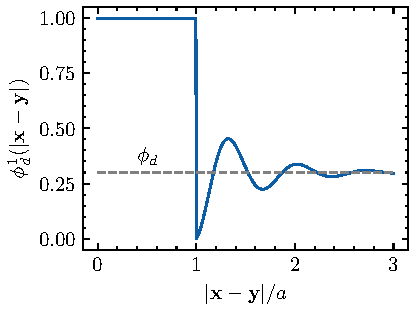
\includegraphics[width=0.2\textheight]{image/dist_phi.pdf}
    \caption{Representation of a possible form for the probability of finding the dispersed phase at \textbf{x} knowing a spherical particle of radius $a$ is present at $\textbf{y}$.
    Note the zone empty of particle concentration near the points $|\textbf{x}- \textbf{y}|=a$, this due to the impenetrability of particles. 
    }
    \label{fig:distrib}
\end{figure}
At the surface of the test-particle, the probability of finding the dispersed phase, i.e. finding the dispersed phase in contact with the surface of the reference particle, is identically null (not to be confused with the probability of finding another droplet center of mass). 
Indeed, a thin film of continuous phase always separates the droplet's surface from its neighbors (see \ref{fig:distrib}).
Therefore, we may write $\phi_d^1 = 0$ at $|\textbf{x}- \textbf{y}| =a$. 
Thus, when evaluated at the subsurface of the particle, we can use the relation $\textbf{u}_f^1 = \textbf{u}^1$ and $p_f^1 = p^1$. 
Consequently, to compute the surface stress of a particle, either the conditionally-averaged quantities of the continuous phase ($\textbf{u}_f^1, p_f^1$) or the bulk quantities ($\textbf{u}^1$, $p^1$) are required. 
Another consequence of this is that, the definitions given by, \ref{eq:sigma_f_surf15}, \ref{eq:sigma_f_surf2}, or \ref{eq:sigma_f_surf} are all consistent when evaluated at the points located on the surface of the droplet at \textbf{x}. 

\subsection{Mean fields and disturbance fields contribution}

As it is often done in the literature \citep{zhang1994ensemble,jackson2000,wang2021numerical,wang2024effect}, we would like to separate the averaged momentum exchange into a contribution from the mean flow and pressure fields, and the contribution arising due to the disturbance velocity and pressure fields.  

\subsubsection{Definitions}

In the first place, we need to define what is a disturbance field.
Let us take the example of the conditioned velocity field, $\textbf{u}_f^1$, and its corresponding disturbance velocity field.
We state that the conditioned field, $\textbf{u}_f^1$, is equivalent to the ensemble-averaged velocity field $\textbf{u}_f$ when the particle at \textbf{x} is sufficiently far from the point where the velocity $\textbf{u}_f^1$ is evaluated (the point \textbf{y}).
Thus, we write,  
\begin{equation}
    \lim_{|\textbf{y}-\textbf{x}|\to\infty} 
    \textbf{u}_f^1[\textbf{y},\textbf{x},\textbf{w},t]
    =
    \textbf{u}_f[\textbf{y},t]. 
    \label{eq:lim_u_1}
\end{equation} 
Note that this definition requires an infinitely large domain. 
This implies that the solutions obtained in the subsequent sections are restricted to infinitely large domains, devoid of boundary conditions.

Let us assume that $L$ is the macroscopic length scale of our process and that $a$  is the typical size of the particles.
Since the particle-size scale $a$ is much smaller than the boundary length scale $L$ we assume that $\textsc{O}(a/L)$ is negligible. 
In the worth case scenario, the disturbance field of a droplet is $(\textbf{u}_f^1- \textbf{u}_f)\sim a/|\textbf{y}-\textbf{x}|$ \citet{kim2013microhydrodynamics}.
Hence, in a physical situation where $|\textbf{y}-\textbf{x}|\to L$ instead of $|\textbf{y}-\textbf{x}|\to\infty$ in \ref{eq:lim_u_1} we may estimate that the error is of $\mathcal{O}(a/L)$, hence negligible upon a reasonable separation of scale.
However, it is interesting to note that this will no longer be the case for other problems such as sediment transport for examples.
In this case, the boundary condition, i.e. the top of the particle bed and the ground, are at a distance of the same length scale as the particle-size. 

In light of \ref{eq:lim_u_1}, we define the disturbance velocity field as 
\begin{equation}
    \textbf{u}_f^{1d}
    =
    \textbf{u}_f^1 
    - 
    \textbf{u}_f. 
    \label{eq:def_u_1d}
\end{equation}
because it satisfies the definition, 
\begin{equation}
    \lim_{|\textbf{y}-\textbf{x}|\to\infty} 
    \textbf{u}_f^{1d}[\textbf{y},\textbf{x},\textbf{w},t]
    =
    \lim_{|\textbf{y}-\textbf{x}|\to\infty} 
    \{\textbf{u}_f^1[\textbf{y},\textbf{x},\textbf{w},t]
    - \textbf{u}_f[\textbf{y},t]\}
    = 0.
    \label{eq:lim_u_1d}
\end{equation} 
Thus, $\textbf{u}_f^{1d}$ tends to zero at large distances from the particle, which is consistent with the terminology ``disturbance''.
The definition \ref{eq:def_u_1d} can apply to any \textit{conditional-averaged} quantities $f^1$, we define
\begin{equation}
    \lim_{|\textbf{y}-\textbf{x}|\to\infty} 
    \{f_f^1[\textbf{y},\textbf{x},\textbf{w},t]
    - f_f[\textbf{y},t]\}
    =
    f_f^{1d}[\textbf{y},\textbf{x},\textbf{w},t]
    = 0.
\end{equation} 

\subsubsection{Momentum exchange decomposition}

Using the decomposition $\bm\sigma_f^1 = \bm\sigma_f^{1d} + \bm\sigma_f$ in \ref{eq:conditionally_averaged} we finally introduce the decomposition of the averaged momentum exchange term as:  
\begin{align}
    \pSavg{\bm\sigma_f^0\cdot\textbf{n}}[\textbf{x},t]
    =
    n_p[\textbf{x},t]
    \int_{|\textbf{x}-\textbf{y}|=a}
    \bm\sigma_f[\textbf{y},t]
    \cdot \textbf{n}
    d\textbf{y}
    \nonumber
    \\
    + 
    \int_{\mathbb{R}^3}
    P_1[\textbf{x},\textbf{w},t]
    \int_{|\textbf{x}-\textbf{y}|=a}
    \bm\sigma_f^{1d}[\textbf{y},\textbf{x},\textbf{w},t]
    \cdot \textbf{n}
    d\textbf{y}
    d\textbf{w}
    \label{eq:general_partition}
\end{align}
where the first term represents the contribution from the mean continuous phase stress, $\bm\sigma_f$, and the second term is the contribution from the disturbance fields stress $\bm\sigma_f^{1d}$. 
While this decomposition is arbitrary since $\bm\sigma_f^1$ could be partitioned into other arbitrary tensors, it enables by definition, the separation of the mean flow contribution, $\bm\sigma_f$, from the stress induced by the local-scale disturbance fields, $\bm\sigma_f^{1d}$.
This decomposition is used by \citet[Chapter 2]{jackson2000} and \citet{zhang1997momentum,wang2021numerical,wang2024effect} for suspensions of solid spheres, although these authors do not explicitly provide the expression for the tensor $\bm\sigma_f^{1d}$, which we aim to derive in the following sections. 

Note that $\bm\sigma_f$ is evaluated at $\textbf{y}$ in \ref{eq:general_partition}. 
Although $\bm\sigma_f$ is ensemble-averaged, we emphasize that it may still depend on the position in inhomogeneous flows. 
Assuming the suspension is slightly non-homogeneous \citep{lhuillier1992ensemble}, we have $\bm\sigma_f[\textbf{y},t] = \bm\sigma_f[\textbf{x},t] + \textbf{r}\cdot \nabla\bm\sigma_f[\textbf{x},t] + \ldots$, where $\textbf{r} = \textbf{y} - \textbf{x}$. 
By retaining only the first three terms in the expansion, we can demonstrate that
\begin{equation}
    \pSavg{\bm\sigma_f^0\cdot\textbf{n}}
    =
    n_p v_p 
    \div\bm\sigma_f
    +
    \int_{\mathbb{R}^3}
    P_1
    \int_{|\textbf{x}-\textbf{y}|=a}
    \bm\sigma_f^{1d} \cdot \textbf{n}
    d\textbf{y}d\textbf{w}.
    \label{eq:drag_final}
\end{equation}
Therefore, the total momentum exchange term contains a component related to the divergence of the mean fluid-phase stress, in addition to the contribution from the disturbance fields. 
Similar arguments can be extended to the first two moments of the hydrodynamic force. 
These expressions can be written as:
\begin{align}
    \pSavg{\textbf{r}\bm\sigma_f^0\cdot\textbf{n}}
    &=
    n_p v_p \bm\sigma_f
    +
    \int_{\mathbb{R}^3}
    P_1
    \int_{|\textbf{x}-\textbf{y}|=a}
    \textbf{r}\bm\sigma_f^{1d} \cdot \textbf{n}
    d\textbf{y}
    d\textbf{w},
    \label{eq:first_mom_general}
    \\
    \pSavg{\textbf{rr}\bm\sigma_f^0\cdot\textbf{n}}
    &=
    n_pv_p  \frac{a^2}{5} 3 [(\div \bm\sigma_f)\bm\delta]^\text{sym}
    +
    \int_{\mathbb{R}^3}
    P_1
    \int_{|\textbf{x}-\textbf{y}|=a}
    \textbf{rr}\bm\sigma_f^{1d} \cdot \textbf{n}
    d\textbf{y}
    d\textbf{w},
    \label{eq:second_mom_general}
\end{align}
where the operator $[\ldots]^\text{sym}$ returns the symmetric part of the arguments. 
It is important to note that the contribution from the mean stress in the second moment of the hydrodynamic force may become negligible when a proper separation of scale is considered. 
Indeed, this term is proportional to $a^2$ \eqref{eq:second_mom_general}, and it appears under the operator $\grad\grad\sim L^{-2}$ in the averaged momentum equation \ref{eq:dt_hybrid_rhou_f}, hence contributing to $\mathcal{O}(a^2/L^2)$, which may be considered as negligible. 

According to the expressions \ref{eq:drag_final}, \ref{eq:first_mom_general}, and \ref{eq:second_mom_general}, we will need to compute the term $\bm\sigma^{1d}_f = \bm\sigma_f^1 - \bm\sigma_f$ where $\bm\sigma_f^1$ is given by \ref{eq:sigma_f_surf}. 
Regarding the mean continuous phase stress we recall that it can be written in two ways (see \ref{chap:daniel15}), namely 
\begin{align}
    \label{eq:mean_continuous_phase_stress}
    \bm\sigma_f
    &= - p_f \bm\delta 
    + \mu_f [\pddy \textbf{u}_f+ (\pddy \textbf{u}_f)^\dagger ]
    - \frac{\mu_f}{\phi_f}\avg{\delta_\Gamma (\textbf{n}_d \textbf{u}_f'+  \textbf{u}_f' \textbf{n}_d)}, \\
    \bm\sigma_f
    &= - p_f \bm\delta 
    + \frac{\mu_f}{\phi_f} [\pddy \textbf{u}+ (\pddy \textbf{u})^\dagger ]
    - \frac{\mu_f \phi_d}{\phi_f} \textbf{e}_d
    \label{eq:mean_continuous_phase_stress2}
\end{align}
Thus using \ref{eq:sigma_f_surf} and \ref{eq:mean_continuous_phase_stress} we find for the points on the particle's surface ($|\textbf{y}-\textbf{x}| = a$) that,
\begin{align}
    \bm\sigma_f^{1d}
    =
    - p_f^{1d} \bm\delta 
    + \mu_f [\pddy \textbf{u}_f^{1d}+ (\pddy \textbf{u}_f^{1d})^\dagger ]
    + \frac{\mu_f }{\phi_f}\avg{\delta_\Gamma (\textbf{n}_d \textbf{u}_f'+  \textbf{u}_f' \textbf{n}_d)}. 
    \label{eq:sigma_explict}
\end{align}
Thus, according to \ref{eq:sigma_explict}, the disturbance stress that is integrated over the particle surface in \ref{eq:drag_final} to \ref{eq:second_mom_general}, is not only the Newtonian stress-like contribution of the disturbance fields ($\textbf{u}_f^1$ and $p_f^1$), but also includes the contribution of the term $\avg{\delta_\Gamma (\textbf{n}_d \textbf{u}_f'+  \textbf{u}_f' \textbf{n}_d)}$. 
Thus, in the force closures: \ref{eq:drag_final} and \ref{eq:first_mom_general}, we will observe the appearance of the terms involving the divergence of $\avg{\delta_\Gamma (\textbf{n}_d \textbf{u}_f'+  \textbf{u}_f' \textbf{n}_d)}$ times $n_pv_p$, and  $n_pv_p \avg{\delta_\Gamma (\textbf{n}_d \textbf{u}_f'+  \textbf{u}_f' \textbf{n}_d)}$, respectively. 
These terms will ultimately cancel out their corresponding contributions in $\bm\sigma_f$ that appear on the left-hand side of \ref{eq:drag_final} and \ref{eq:first_mom_general}. 

To provide a better understanding for the following discussion we remark that for solid particles $\textbf{e}_d = 0$. 
Therefore, subtracting \ref{eq:mean_continuous_phase_stress} from \ref{eq:mean_continuous_phase_stress2}, directly gives, 
\begin{equation}
    \avg{\delta_\Gamma (\textbf{n}_d \textbf{u}_f'+  \textbf{u}_f' \textbf{n}_d)}
    = 
    (\textbf{u}_f - \textbf{u}_d)\pddy \phi_d + \pddy \phi_d (\textbf{u}_f - \textbf{u}_d)
    -  \phi_d [\pddy \textbf{u}_d+ (\pddy \textbf{u}_d)^\dagger ]. 
    \label{eq:closure_un_nu}
\end{equation} 
Therefore, at least for solid particles, this term is non-zero as soon as there are non-negligible gradients of volume fraction and mean gradients of particle velocities. 


We conclude that the commonly used decomposition of the drag force introduced by \citet{zhang1997momentum,jackson2000}, given by \ref{eq:general_partition}, requires adding the term  $\avg{\delta_\Gamma (\textbf{n}_d \textbf{u}_f'+  \textbf{u}_f' \textbf{n}_d)}$ to the classical Newtonian stresses in the second term of \ref{eq:general_partition} and subtracting it in the mean drag force term (first term of \ref{eq:general_partition}). 
This finding implies that, in the recent work of \citet{wang2021numerical, wang2024effect}, where this decomposition is employed for the drag force, we assert that they have actually computed the integral of the first two terms of \ref{eq:sigma_explict}, while neglecting the final term. 
Interestingly, \citet{wang2024effect} specifically investigates the effect of the volume fraction gradient ($\grad \phi_d$) on the drag force. 
In this context, it is clear from \eqref{eq:closure_un_nu} that the term $\avg{\delta_\Gamma (\textbf{n}_d \textbf{u}_f'+  \textbf{u}_f' \textbf{n}_d)}$ cannot be neglected. 
Only when the analysis is accurate to $\mathcal{O}(\phi_d)$ does this term vanish in \ref{eq:drag_final}, reducing \ref{eq:sigma_explict} to the Newtonian stress expression. 
% Thus, the drag force computed in the DNS of \citet{wang2024effect} may not be the one defined in their momentum equations. 

Note that using \ref{eq:mean_continuous_phase_stress2} instead of \ref{eq:mean_continuous_phase_stress} in \ref{eq:sigma_explict} and switching $\textbf{u}_f^1$ and $\textbf{u}^1$ in \ref{eq:sigma_f_surf}, does not solve this inconsistency. 

\subsubsection{An alternative stress decomposition}

As the previous decomposition requires adding and subtracting $\avg{\delta_\Gamma (\textbf{n}_d \textbf{u}_f'+  \textbf{u}_f' \textbf{n}_d)}$ in each term of \ref{eq:general_partition}, we decide to avoid this overcomplicated operation and introduce, the partitioning 
\begin{equation}
    \bm\sigma_f^1 =
    \bm\Sigma_f + 
    \bm\Sigma_f^{1d}. 
    \label{eq:mean_Newtonian}
\end{equation}
Where the mean stress and disturbance stresses are defined as, 
\begin{align}
    \bm\Sigma_f^{1d}
    &=-p_f^{1d}\bm\delta + \mu_f^1 [\grad \textbf{u}^{1d}_f + (\grad \textbf{u}^{1d}_f)^\dagger], \\
    \bm\Sigma_f
    &=-p_f\bm\delta + \mu_f^1 [\grad \textbf{u}_f + (\grad \textbf{u}_f)^\dagger], 
\end{align}
respectively. 
Note that the use of $\textbf{u}_f$ as the ensemble-averaged velocity of reference is arbitrary.
Indeed, recall that at the surface of the test particle we have $\phi_d^1=0$, hence $\textbf{u}_f^1 = \textbf{u}^1$. 
Thus, at the surface of the test-particle, one could use the decomposition,
\begin{equation}
    \bm\sigma_f^1 =
    \bm\Sigma + 
    \bm\Sigma^{1d}. 
    \label{eq:mean_Newtonian2}
\end{equation}
Where the mean stress and disturbance stresses are defined as, 
\begin{align}
    \bm\Sigma^{1d}
    &=-p_f^{1d}\bm\delta + \mu_f^1 [\grad \textbf{u}^{1d} + (\grad \textbf{u}^{1d})^\dagger], \\
    \bm\Sigma
    &=-p_f\bm\delta + \mu_f^1 [\grad \textbf{u} + (\grad \textbf{u})^\dagger]. 
\end{align}
One could wonder which of these stress decomposition (\ref{eq:mean_Newtonian2} or \ref{eq:mean_Newtonian}) is the more efficient? 
The answer is that it depends on the unknown of the problem at hand. 
If we consider an averaged system of equations for the mean continuous phase field $\textbf{u}_f$ then, \ref{eq:mean_Newtonian} seems more adapted, however, if the unknown is \textbf{u}, then \ref{eq:mean_Newtonian2} is more adapted. 
In all case since $\textbf{u} = \textbf{u}_f + \phi_d (\textbf{u}_d - \textbf{u}_f)$ one can always recover \ref{eq:mean_Newtonian2} from \ref{eq:mean_Newtonian} or inversely.




Using the same methodology as in the previous manipulations we re-write the force closures as, 
\begin{align}
    \pSavg{\bm\sigma_f^0\cdot\textbf{n}}
    &=
    n_p v_p 
    \div\bm\Sigma_f
    +
    \int_{\mathbb{R}^3}
    P_1
    \int_{|\textbf{x}-\textbf{y}|=a}
    \bm\Sigma_f^{1d} \cdot \textbf{n}
    d\textbf{y}d\textbf{w}
    \label{eq:drag_final2}\\
    \pSavg{\textbf{r}\bm\sigma_f^0\cdot\textbf{n}}
    &=
    n_p v_p \bm\Sigma_f
    +
    \int_{\mathbb{R}^3}
    P_1
    \int_{|\textbf{x}-\textbf{y}|=a}
    \textbf{r}\bm\Sigma_f^{1d} \cdot \textbf{n}
    d\textbf{y}
    d\textbf{w}
    \\
    \pSavg{\textbf{rr}\bm\sigma_f^0\cdot\textbf{n}}
    &=
    n_pv_p  \frac{a^2}{5} 3 [(\div \bm\Sigma_f)\bm\delta]^\text{sym}
    +
    \int_{\mathbb{R}^3}
    P_1
    \int_{|\textbf{x}-\textbf{y}|=a}
    \textbf{rr}\bm\Sigma_f^{1d} \cdot \textbf{n}
    d\textbf{y}
    d\textbf{w}
    \label{eq:second_mom_general2}
\end{align}
This decomposition, though perhaps less natural, appears to be more physically meaningful. 
Indeed, unlike the previous approach, the mean contribution no longer depends on the mean relative motion through the term $\avg{\delta_\Gamma (\textbf{n}_d \textbf{u}_f'+  \textbf{u}_f' \textbf{n}_d)}$ in $\bm\sigma_f$ (see \ref{eq:closure_un_nu}), but solely on the mean fluid phase properties $p_f$ and $\textbf{u}_f$, while the local stress is a Newtonian-like stress.  

The main take-away of this section is that: (1)  the particle-averaged force traction terms can be computed based on the knowledge of $p_f^{1d}$ and $\textbf{u}_f^{1d}$. 
These fields can be obtained by solving the corresponding disturbance field equations. 
Note that one may also compute the mixture properties $p^{1d}$ and $\textbf{u}^{1d}$ and then use the relation $p_f^{1d} = p^{1d} + \phi_d (p_f - p_d)$ or $\textbf{u}_f^{1d} = \textbf{u}^{1d} + \phi_d (\textbf{u}_f - \textbf{u}_d)$. 
And (2) the force decomposition often used \citep{jackson2000,zhang1997momentum,wang2021numerical,wang2024effect} seems inconsistent compared to the drag force computed in the cited studies.
Indeed, it is likely that their definition of the ``drag force'' term, requires the subtraction of a term proportional to the particle volume fraction. 
This inconsistency is settled by re-defining the forces partition.  

\subsection{Particle phase volumic terms}

Some closure terms such as the particle internal stress $\pOavg{\bm{\sigma}_2^0}$ or the particle internal dissipation term $\pOavg{\bm{\sigma}_2^0:\grad \textbf{u}_d^0}$ are particle-averaged volume integral of locals quantities. 
In this situation the reformulation is slightly different since we must consider volume and not the surfaces of the particle.  Nevertheless the approach is similar. 
For the particle internal stress we can write, 
\begin{equation}
    \pOavg{\bm\sigma_d^0}[\textbf{x},t]
    =
    \int_{\mathbb{R}^3}
    P_1[\textbf{x},\textbf{w}]
    \int_{|\textbf{x}-\textbf{y}|<a}
    \bm\sigma_d^1[\textbf{y},t;\textbf{x},\textbf{w}] 
    d\textbf{y}
    d\textbf{w}. 
    \label{eq:conditionally_averaged_vol}
\end{equation}
Assuming a Newtonian fluid for the particles, $\bm\sigma_d^0 = -p_d^0 \bm\delta + \mu_d [\nabla \textbf{u}_d^0 + (\nabla \textbf{u}_d^0)^\dagger]$, and given that within the region $|\textbf{x} - \textbf{y}| < a$, only the dispersed phase is present.
This allows the permutation between ensemble averages and derivatives.
We can express this as:
\begin{equation}
    \bm\sigma_d^1  
    = 
    -p_d^1   \bm\delta
    + \mu_d  [\pddy \textbf{u}^1_d+(\pddy  \textbf{u}^1_d)^\dagger],
    \label{eq:dispersed_phase_stress}
\end{equation}
which is simply the expression of the Newtonian stress within the particle centered at \textbf{x}, based on the mean fields $p_d^1$ and $\textbf{u}_d^1$. 
As in the previous section, one can eventually partition this conditional stress into an ensemble averaged stress plus a local disturbance field. 

\subsection{Continuous phase closures}

The closure terms of the form $\avg{\chi_f f_f^0}$ differ in their mathematical structure, as they represent an average over the continuous phase rather than the dispersed phase. 
Consequently, the reformulation method is slightly different and requires additional assumptions. Two examples of such terms are the Reynolds stress $\avg{\chi_f \textbf{u}_f'\textbf{u}_f'}$ and the fluid-phase dissipation $\avg{\chi_f \bm\sigma_f^0 : \nabla \textbf{u}_f^0}$, which appear in \ref{eq:dt_hybrid_rhou_f} and \ref{eq:dt_hybrid_k1}, respectively.  

We first note that, 
\begin{equation}
    \frac{1}{N}\sum_\alpha^N
    \int_{\mathbb{R}^3}
    \int_{\mathbb{R}^3}
    \delta(\textbf{y}-\textbf{x}_\alpha[\FF,t])
    \delta(\textbf{w}-\textbf{u}_\alpha[\FF,t])
    d\textbf{x}
    d\textbf{w}
    = 1,
\end{equation}
where $N$ is the total number of particles in the flow. 
Using this relation one may re-formulate the ensemble average of a continuous phase quantity as 
\begin{equation}
    \phi_f f_f[\textbf{x},t]
    = 
    \frac{1}{N}
    \int_{\mathbb{R}^3}
    \int_{\mathbb{R}^3}
    f_f^1[\textbf{x},\textbf{y},\textbf{w},t] \phi_f^1[\textbf{x}|\textbf{y},\textbf{w},t]  P_1[\textbf{y},\textbf{w}] 
    d\textbf{y} 
    d\textbf{w}
    \label{eq:conditional_averaged_fluid}
\end{equation}
where,
\begin{equation*}
    f_f^1[\textbf{x},\textbf{y},\textbf{w},t] \phi_f^1[\textbf{x}|\textbf{y},\textbf{w},t]  P_1[\textbf{y},\textbf{w}]
    =     
    \avg{
    \sum_\alpha^N 
    \delta(\textbf{y}-\textbf{x}_\alpha[\FF,t])
     \delta(\textbf{w}-\textbf{u}_\alpha[\FF,t])
    (\chi_f
    f^0_f)[\textbf{x},t;\FF]
    }.
\end{equation*}
In this expression $f_f^1[\textbf{x},t;\textbf{y},\textbf{w}]$ is the average of the local quantity $f_f^0$ evaluated at $\textbf{x}$ and time $t$ conditionally on, the presence of the continuous phase at \textbf{x}, and a particle center of mass at $\textbf{y}$ with center of mass velocity $\textbf{w}$. 
Similarly, $\phi_f^1[\textbf{x},t|\textbf{y},\textbf{w}]$ is the fluid phase volume fraction at \textbf{x} and time $t$, conditionally on the presence of a particle at $\textbf{y}$ with center of mass velocity \textbf{w}. 
Note that for $|\textbf{x} - \textbf{y}| < a$, $\phi_f^1[\textbf{y}|t,\textbf{x},\textbf{w}] = 0$ however at, 
$\lim_{|\textbf{x} - \textbf{y}| \to \infty} \phi_f^1 = \phi_f$. 
Note that this derivation is consistent with (2.21) and (2.22) of \citet{zhang1994ensemble} with $K = 1$. 

This, formulation remains quite general and is valid regardless of the flow regime, however, the presence of the term $N$ makes this formulation unpractical. 
Indeed, $P_1 = n_p[\textbf{y},t] P_1[\textbf{w}|\textbf{y},t]$ and $n_p[\textbf{y},t] /N = V_\Omega$, where $V_\Omega$ is the volume of the whole domain. 
Thus, substituting  $n_p[\textbf{y},t] /N = V_\Omega$ into \ref{eq:conditional_averaged_fluid} transforms the right-hand side of this relation to a volume average over $V_\Omega$ of a property evaluated at \textbf{x} on all possible particles positions in $V_\Omega$.  
Anyhow, \ref{eq:conditional_averaged_fluid} requires macroscopic information such as $N$ and $V_\Omega$, which we do not necessarily have if our goal is to compute general closure formulation. 
This is because, contrary to particle-averaged quantities, we could not consider a contribution per particle that is holds fixed at \textbf{x}, but the action of all particles on a given property of the fluid at \textbf{x}.
In other words, the integration variable is on the particle center of mass position in \ref{eq:conditional_averaged_fluid}, while in \ref{eq:conditionally_averaged} it is on the local non-averaged properties while the particle position remains fixed. 

Consequently, we adopt the approach proposed by \citet{batchelor1972sedimentation} and reformulate \ref{eq:conditional_averaged_fluid} based on the additivity assumption \footnote{
    This implicitly assumes that $f_f^0$ is governed by a linear equation. 
    That is the case for the Stokes flow regime, or unsteady Stokes flow regime if $f_f^0$ is the velocity. 
}. 
Thus, we postulate that $f_f^0[\textbf{x},t;\FF]$ can be subdivided into $N$ contributions, namely:  
\begin{equation}
    f_f^0[\textbf{x},t;\FF]
    = 
    \sum_\alpha^N
    f_{f_\alpha}^0[\textbf{x},t;\FF]
    + f_{f_0}^0[\textbf{x},t;\FF]
\end{equation}
where $f_{f_\alpha}^0$ is the disturbance fields produced by the particle $i$ on $f_f^0$ and $f_{f_0}^0$ is the undisturbed background flow. 
This implies that $f_{f}^0 = f_{f_0}^0$ in the absence of particle in the flow. 
Under this assumption, we can write, 
\begin{equation}
    \avg{\chi_f f_f^0}[\textbf{x},t]
    = 
    \int_{\mathbb{R}^3} 
    \avg{
        \sum_\alpha^N 
    (\chi_f f_{f_\alpha}^0)[\textbf{x}_\alpha + \textbf{r},t,\FF] \delta(\textbf{x} - \textbf{x}_\alpha[\FF,t] - \textbf{r})}d\textbf{r}
    +( \phi_f f_{f_0})[\textbf{x},t]
    \label{eq:first_step_additivity}
\end{equation}
Where $\phi_f f_{f_0}[\textbf{x},t]$ is the mean background flow, and were we have used a relation similar to the one presented in \ref{app:expansion}, to reformulate the first term of \ref{eq:first_step_additivity}. 
Then, we use the Taylor expansion, $\delta(\textbf{x} - \textbf{x}_\alpha - \textbf{r}) =\delta(\textbf{x} - \textbf{x}_\alpha) - \textbf{r}\cdot \grad\delta(\textbf{x} - \textbf{x}_\alpha)+ \ldots$, on the first term on the right-hand side of \ref{eq:first_step_additivity}.
This gives,  
\begin{align}
    \avg{\chi_f f_f^0}[\textbf{x},t]
    = 
    \phi_f f_{f_0}[\textbf{x},t]
    + 
    \int_{\mathbb{R}^3} 
    \int_{\mathbb{R}^3} 
    (f_{f_p}^1\phi_f^1) [\textbf{y}|\textbf{x},\textbf{w},t] P_1[\textbf{w},\textbf{x}]
    d\textbf{r}
    d\textbf{w}
    \nonumber \\
    + 
    \div 
    \int_{\mathbb{R}^3} 
    \int_{\mathbb{R}^3} 
    \textbf{r}
    (f_{f_p}^1\phi_f^1) [\textbf{y}|\textbf{x},\textbf{w},t] P_1[\textbf{w},\textbf{x}]
    d\textbf{r}
    d\textbf{w}
    + \ldots
    % + \grad^n 
    % \int_{\mathbb{R}^6} 
    % \mathcal{O}(\textbf{r}^n)
    % (f_{f_p}^1\phi_f^1) [\textbf{y}|\textbf{x},\textbf{w},t] P_1[\textbf{w},\textbf{x}]
    % d\textbf{r}
    % d\textbf{w}
    \label{eq:f_f_1_def}
\end{align}
with, 
\begin{equation}
    (f_{f_p}^1 \phi_f^1) [\textbf{y}|\textbf{x},\textbf{w},t] P_1[\textbf{w},\textbf{x}]
    = 
    \avg{
    \sum_\alpha
    \chi_f f_{f_\alpha}^0[\textbf{x}_\alpha + \textbf{r},t;\FF] 
    \delta(\textbf{x} - \textbf{x}_\alpha[\FF,t])
    \delta(\textbf{w} - \textbf{u}_\alpha[\FF,t])
    }. 
\end{equation}
In this definition $f_{f_p}^1$ is the averaged value of the disturbance fields at $\textbf{x}+\textbf{r}$, produced by the particle at $\textbf{x}$, in opposition to $f_f^1$ \eqref{eq:conditional_averaged_fluid} which is the averaged value of $f_f^0$ evaluated at \textbf{x}, conditionally on the presence of an arbitrary particle at \textbf{y}.
Assuming a situation where there is no background flow (such as in the case of sedimenting particle in an otherwise quiescent flow), a homogeneous situation, and in the dilute limit, such that $\phi_f^1 = \phi_f$ when $|\textbf{x}-\textbf{y}|>a$ and $\phi_f^1 =0$ when $|\textbf{x}-\textbf{y}|<a$, we obtain, 
\begin{equation}
    f_f[\textbf{x},t]
    = 
    \int_{\mathbb{R}^3} 
    P_1[\textbf{x},\textbf{w}] 
    \int_{|\textbf{x}-\textbf{y}| >a} 
    f_{f_p}^1[\textbf{x}+ \textbf{r}| \textbf{x}]
    d\textbf{r}
    d\textbf{w}
    + 
    \text{Error}
    \label{eq:Batchelor2}
\end{equation}
\begin{equation}
    \text{Error}
    = 
    \int{
    \mathcal{O}(|\textbf{r}| f_{f_p}^1  n_p / L)
    } d\textbf{r}. 
    \label{eq:error0}
\end{equation}
Note that in \ref{eq:error0} we have expressed explicitly the error generated due to the Taylor expansion of the Dirac delta: $\delta(\textbf{x} - \textbf{x}_\alpha - \textbf{r})$. 
Indeed, at the leading order we find, $\delta(\textbf{x} - \textbf{x}_\alpha - \textbf{r}) =\delta(\textbf{x} - \textbf{x}_\alpha) +  \mathcal{O}(|\textbf{r}|/L)$, where $L$ is the typical length of the macroscopic flow variation.
Assuming that $\text{Error}= \mathcal(\phi_d^2)$ rather than \ref{eq:error0} in \ref{eq:Batchelor2}, we find that \ref{eq:Batchelor2} is exactly equation (2.10) of \citet{batchelor1972sedimentation}. 
\citet{batchelor1972sedimentation} uses such a formula to compute the mean fluid phase velocity at a given point in the fluid, conditionally on the presence of a particle at a certain distance from this point. 
Consequently, \ref{eq:Batchelor2} provides an extension of Eq (2.10) of \citet{batchelor1972sedimentation}, in the sense that we give an explicit expression of the``Error'' term \eqref{eq:error0}. % based on mathematical arguments, rather than Batchelor's physical arguments. 
Additionally, \ref{eq:f_f_1_def} is a generalization of \ref{eq:Batchelor2} when the homogeneous hypothesis, as well as the dilute hypothesis, are not assumed. 



As discussed in \citet{batchelor1972sedimentation}, the first integral in \ref{eq:f_f_1_def} may diverge if the disturbance field $f_{f_p}^1$ does not decay rapidly enough as $|\textbf{r}|$ approaches infinity. 
We believe that, in cases where $f_{f_p}^1$ does not decay sufficiently fast as $|\textbf{r}|$ increases, the ``Error'' in \ref{eq:Batchelor2} also tends to infinity since we integrate a term proportional to $f_{f_p}^1 |\textbf{r}|$ which is even more divergent for large $|\textbf{r}|$. 
Thus, we argue that Batchelor's original formula is not accurate at $\mathcal{O}(\phi_d^2)$, but rather at $\mathcal{O}(|\textbf{r}| f_{f_p}^1  n_p / L)$, making \ref{eq:Batchelor2} unable to produce physical results when $f_{f_p}^1$ does not decay rapidly since the ``Error'' also tends to infinity in these cases. 
In cases where the first integral on the right-hand side converges, but the "Error" does not, the results must still be considered with caution, though the first integral is. 


Additionally, we believe that in the general case, where $f_f$ is given by \ref{eq:f_f_1_def}, it is impossible to obtain meaningful results with the latter formula. 
Indeed, \ref{eq:f_f_1_def} requires the use of the Taylor expansion, $\delta(\textbf{x} - \textbf{x}_\alpha - \textbf{r}) =\delta(\textbf{x} - \textbf{x}_\alpha) - \textbf{r}\cdot \grad\delta(\textbf{x} - \textbf{x}_\alpha)+ \ldots + \mathcal{O}(\textbf{r}^n/L^n)$. 
Additionally, in the integrals of \ref{eq:f_f_1_def}, \textbf{r} is evaluated from the particle center to an infinitely large distance from it.
Thus, it is evident that for any unbounded $f_{f_p}^1$, when $|\textbf{r}| \to \infty$, there is always an arbitrary integer $n$ for which, $\int f_{f_p}^1 \phi^1_f \textbf{r}^n d\textbf{r} \to \infty$.
Thus, if one considers a sufficiently high order moment in \ref{eq:f_f_1_def}, he will end up including a divergent integral. 
Following the same argument we can show that the  ``Error'' term included due to the Taylor expansion, proportional to $\mathcal{O}(f_{f_p}^1 r^n /L^n)$ might diverge as well since $r$ goes to infinity and $L$ stays constants. 
Consequently, in the inhomogeneous situations, and for unbounded functions $f_{f_p}^1$, we state that \ref{eq:f_f_1_def} might be not relevant as it produces divergent integral and an infinite ``Error'' as well. 

Note that the wake of a spherical particle in an unbounded fluid in Stokes flow, yields a velocity field $\textbf{u}_{f_p}$ proportional to  $\sim 1/|\textbf{r}|$. 
Thus, such a velocity field is a good example of a situation where: the continuous phase properties $f_{f_p}^1$ is unbounded, the first integral and the ``Error'' in \ref{eq:Batchelor2} diverge. 
In such cases, Batchelor used the renormalization method to circumvent these difficulties. 
% Note that these problems of divergent integral could be guessed well in advance since the Taylor expansion of $\delta(\textbf{x} - \textbf{x}_\alpha - \textbf{r})$ for a vector $\textbf{r}$ that is arbitrarily large doesn't make
% Nevertheless, such manipulation is required to demonstrate Batchelor's original formula and its generalization given by \eqref{eq:Batchelor2}. 


 
In conclusion, \ref{eq:Batchelor2}  is meaningful only for fields that respect the following conditions: 
(1) The influence of the particles on the field $f_f^0$ must be additive, this is the case when ${f_f^0}$ follows the Stokes equations; 
(2) The closures must be derived in a homogeneous flow, such that the higher moments in \ref{eq:f_f_1_def} cancel exactly. 
And (3), the integral over $\mathbb{R}^3$ of the term $|\textbf{r}| f_{f_p}^1$ must be finite, such that \ref{eq:Batchelor2} remains finite. 
Even if \ref{eq:Batchelor2} is not ideal, we will be using this relation to compute the continuous phase closures since for instance, this is the only tool that we have. 
Note that a new method will be presented in \ref{chap:pseudoturbulence} where we use \textit{The Nearest particle statistics} \citep{zhang2021ensemble} to compute these kinds of ensemble-averaged terms, but without the need for such approximations.


\section{Single-particle ensemble averaged problem}
\label{sec:the_disturbance_eq}

Now that we have proved the link between the ensemble-averaged closures and the conditional averaged quantities, we present the corresponding equations for these averaged conditional quantities. 
For all the closure related to the momentum equations, we need to find: $\textbf{u}^{1d}$ and $p^{1d}$ or $\textbf{u}^{1d}_f$ and $p^{1d}_f$. 
To that end, we follow \citep{hinch1977averaged,zhang1994averaged} and derive the \textit{single-particle} conditioned Navier-Stokes equations.
It turns out that deriving the \textit{single-particle} conditioned Navier-Stokes equations in a form like \ref{eq:dt_avg_rhou} is considerably simpler than using the \textit{Favre} averaged formulation or two-fluid formulation. 
Thus, in the following, we provide a set of equations for $\textbf{u}^{1d}$ and $p_f^{1d}$. 

We recall that the \textit{single-fluid} formulation of the Navier-Stokes equations, can be written at the local scale as (see \ref{ap:momentum_formulation}),
\begin{align}
    \label{eq:dt_local_mass}
    \div \textbf{u}^0 = 0, \\
    \pddt \textbf{u}^0
    + \div (\textbf{u}^0\textbf{u}^0 - \bm\sigma^*)
    &= \textbf{g}
    +(\kappa/\rho_f)(\bm\sigma_f^0\cdot \textbf{n})\delta_\Gamma,
    \label{eq:dt_local}
\end{align}
Where we noted $\textbf{u}^0 = \chi_f \textbf{u}f^0 + \chi_d \textbf{u}_d^0$, and $\bm\sigma^* = (\chi_f \bm\sigma_f^0 + \chi_d \bm\sigma_d^0/\zeta + \delta_\Gamma \bm\sigma_\Gamma^0/\zeta )/\rho_f $ referred as the density-weighted stress.
$\bm\sigma_{f,d}^0 = -p_{f,d}^0\bm\delta + \mu_{f,d}\left[\grad \textbf{u}_{f,d}^0+ (\grad \textbf{u}_{f,d}^0)^\dagger\right]$ denote the Newtonian stresses and $\bm\sigma_\Gamma^0 = \gamma (\bm\delta - \textbf{nn})$ represents the surface tension stress. 
We introduced $\kappa = (1-\zeta)/\zeta$ and $\zeta = \frac{\rho_d}{\rho_f}$ as the density ratio, consequently the interface exchange term vanishes for iso-dense suspensions. 
The boundary conditions at the surface of the droplets are implicitly included in the \textit{single-fluid} formulation \eqref{eq:dt_local}; however, it will be useful to recall them here for later reference, 
\begin{align}
    \label{eq:dt_rho_I3}
    \textbf{u}_f^0 = \textbf{u}_d^0 = \textbf{u}_\Gamma^0, \\
    \Jump{\bm{\sigma}_k^0} 
    =
    -\gamma\textbf{n}(\div \textbf{n}). 
    \label{eq:dt_rho_I2}
\end{align}

To obtain an equation for the disturbance velocity fields $\textbf{u}^{1d}$ we remark that this field can be defined by the operation, 
\begin{equation}
    \avg{(\delta_1 - P_1) \textbf{u}^0}
    =
    \avg{\delta_1 \textbf{u}^0}
    - \avg{P_1 \textbf{u}^0}
    = 
    P_1 \textbf{u}^1
    - P_1 \textbf{u}
    = P_1 \textbf{u}^{1d}. 
    \label{eq:first_step_u0}
\end{equation}
Note that $\textbf{u}^0$ and \ref{eq:dt_local} are evaluated at the point \textbf{x} while the Dirac function, 
\begin{equation}
    \delta_1[\textbf{y},\textbf{w},t,\FF] = \sum_\alpha^N \delta(\textbf{x}_\alpha[\FF,t]-\textbf{y})\delta(\textbf{u}_\alpha[\FF,t] - \textbf{w}),
\end{equation}
expresses the condition of having a particle at \textbf{y} with velocity \textbf{w}, and is therefore independent of \textbf{x}. 
In opposition to the definition given by \ref{eq:delta_1} we now consider that the particle center of mass is at \textbf{y}. 
From \ref{eq:first_step_u0}, we deduce that the momentum conservation equation for $\textbf{u}^{1d}$ is obtained by multiplying \ref{eq:dt_local} by $\delta_1 - P_1$ and averaging over all configurations. 
However, since $\delta_1$ is still a function of time $t$, this operation will require a conservation equation for $\delta_1$ and $P_1$ as well.  

Taking the partial time derivative of $\delta_1$ yields directly the relation, 
\begin{equation}
    \pddt\delta_1 
    + \pddy\cdot(\textbf{w}\delta_1)
    + \pddw\cdot(\textbf{a}_\alpha\delta_1)
    = 0 
    \label{eq:dt_delta_1}
\end{equation}
where $\textbf{a}_\alpha[\FF,t] = \pddt \textbf{u}_\alpha[\FF,t]$ is the acceleration of the particle $i$ in the configuration $\FF$. 
Ensemble averaging this equation yields an equation for  $P_1[\textbf{x},\textbf{w},t]$ which reads, 
\begin{equation}
    \pddt P_1
    + \pddy\cdot(\textbf{w}  P_1)
    + \pddw\cdot(\textbf{a}_p P_1)
    = 0.
    \label{eq:dt_P_1}
\end{equation}
Where $\textbf{a}_p = \avg{\delta_1 \textbf{a}_\alpha}/P_1$ is the mean acceleration of the center of mass of velocity \textbf{w}. 
This equation is a conservation equation of the one-point statistics: $P_1$,  along its phase space formed by $\textbf{y},\textbf{w},t$. 
Note that integrating \ref{eq:dt_P_1} over $\textbf{w}$ yields a conservation equation for the number density $n_p[\textbf{y},t]$, because of \ref{eq:Pw_normed}.  

\subsection{Single-particle conditionally averaged  Navier-Stokes equations}

% \tb{
%     If $\delta_1$ wheer express in terms of $x + r$ instead? 
%     \begin{align}
%         \pddt (P_1 \textbf{u}^{1d})
%         + \div \avg{(\textbf{u}^0 \textbf{u}^0 - \bm\sigma^*)(\delta_1 - P_1)} 
%         + \div \avg{(\delta_1 - P_1)\textbf{u}^0 \textbf{w}}\nonumber \\ 
%         + \pddw\cdot \avg{(\delta_1\textbf{a}_\alpha - P_1\textbf{a}_p) \textbf{u}^0}
%         =  (\kappa / \rho_f) \avg{ (\delta_1 - P_1) \delta_\Gamma \bm\sigma_f^0\cdot \textbf{n}},
%         + \avg{(\textbf{u}^0 \textbf{u}^0 - \bm\sigma^*)\cdot \grad(\delta_1 - P_1) }
%     \end{align}
% }

Multiplying \ref{eq:dt_local_mass} and \ref{eq:dt_local} by $(\delta_1 - P_1)$ and using \ref{eq:dt_delta_1},  \ref{eq:dt_P_1} yields the general form of the \textit{single-particle} conditionally-averaged \textit{single-fluid} formulation of the Navier-Stokes equations, namely,  
\begin{align}
    P_1 \div \textbf{u}^{1d}
    = 0 
    \label{eq:conditional_eqs_mass}
    \\
    \pddt (P_1 \textbf{u}^{1d})
    + \div \avg{(\textbf{u}^0 \textbf{u}^0 - \bm\sigma^*)(\delta_1 - P_1)} 
    + \pddy\cdot\avg{(\delta_1 - P_1)\textbf{u}^0 \textbf{w}}\nonumber \\ 
    + \pddw\cdot \avg{(\delta_1\textbf{a}_\alpha - P_1\textbf{a}_p) \textbf{u}^0}
    =  (\kappa / \rho_f) \avg{ (\delta_1 - P_1) \delta_\Gamma \bm\sigma_f^0\cdot \textbf{n}},
    \label{eq:conditional_eqs}
\end{align}
We can observe that the only differences with \ref{eq:conditional_eqs} and \ref{eq:conditional_eqs_mass} and their local counterpart is the presence of the factor $(\delta_1 - P_1)$ in front of all the terms, (which represent the constraint of having a particle at \textbf{y}), and the additional advecting terms on the left-hand side of \ref{eq:conditional_eqs}. 
Note that the gravity acceleration term canceled out in \ref{eq:conditional_eqs} since $\avg{(\delta_1 - P_1)\textbf{g}} = (P_1 -P_1 )\textbf{g} =0$. 
This simply means that in the reference frame of $\textbf{u}^{1d}$ the gravity acceleration does not play any role.
This is easily explained, as \ref{eq:conditional_eqs} represents the momentum equation for $\textbf{u}^{1}$, minus the one for $\textbf{u}$, both of which are subject to the body force \textbf{g}.
Even though the goal is not to solve \ref{eq:conditional_eqs} in all its generality, reformulating the terms in \ref{eq:conditional_eqs} and \ref{eq:conditional_eqs_mass} can be useful for gaining physical insight. 


Although we did not explicitly write all the terms of \ref{eq:conditional_eqs} and \ref{eq:conditional_eqs_mass} yet, we can already note some interesting features. 
First, using \ref{eq:examples1},  \ref{eq:conditional_eqs_mass} can be written as $P_1 \div \textbf{u}^{1d} =0$, indicating that the averaged bulk disturbance field around the particle is divergence-free.  

\subsubsection{Advecting terms}

We begin by reformulating the advecting terms of \ref{eq:conditional_eqs}.
Using the definition of $\textbf{u}^{1d}$ we can write, 
\begin{align}
    \label{eq:examples1}
    \avg{(\delta_1 - P_1) \textbf{u}^0}
    &= P_1 \textbf{u}^{1d},\\ 
    \avg{(\delta_1 - P_1)\textbf{u}^0 \textbf{w}}
    &= \avg{(\delta_1 - P_1)\textbf{u}^0 }\textbf{w} 
    = P_1\textbf{u}^{1d}\textbf{w} \\
    \label{eq:examples2}
    \avg{(\delta_1 - P_1)\textbf{u}^0 \textbf{u}^0}
    &= 
    P_1 (\textbf{u}^1\textbf{u}^1 - \textbf{u}\textbf{u})
    + \avg{\delta_1 \textbf{u}''\textbf{u}''}
    - P_1 \avg{ \textbf{u}'\textbf{u}'}
    \nonumber\\
    &= 
    P_1 (\textbf{u}^{1d}\textbf{u}^{1d} + \textbf{u}\textbf{u}^{1d}+  \textbf{u}^{1d}\textbf{u})
    + \avg{\delta_1 \textbf{u}''\textbf{u}''}
    - P_1 \avg{ \textbf{u}'\textbf{u}'}
    \\
    \avg{(\delta_1\textbf{a}_\alpha - P_1\textbf{a}_p) \textbf{u}^0}
    &=
    P_1\textbf{a}_p \textbf{u}^{1d}
    + \avg{\delta_1\textbf{a}_\alpha' \textbf{u}^0} 
    % \\
    % \rho_f \avg{(\delta_1 - P_1) \bm\sigma^*} 
    % &= 
    % \avg{(\delta_1 - P_1) [\chi_f \bm\sigma^0_f]} 
    % \avg{(\delta_1 - P_1) [\chi_d \bm\sigma^0_d +\delta_\Gamma \bm\sigma_\Gamma^0]/\zeta } 
    \label{eq:examples}
\end{align}
We recall that $\textbf{u}'' = \textbf{u}^0 - \textbf{u}^1$, thus the terms $\avg{\delta_1 \textbf{u}''\textbf{u}''}$ corresponds to the fluctuations of the velocity at \textbf{x} over all configuration where a particle is at \textbf{y} with velocity \textbf{w}, while $\avg{ \textbf{u}'\textbf{u}'}$ is the classic \textit{Reynolds stress} tensor evaluated at \textbf{x}. 
Similarly, $\avg{\delta_1\textbf{a}_\alpha' \textbf{u}^0}$ is the covariance between the particle center of mass acceleration located at \textbf{y} and the local bulk velocity evaluated at \textbf{x}. 



In \ref{eq:examples} we can observe the presence of the conditional field $\textbf{u}^{1d}$ and the ensemble-averaged velocity $\textbf{u}$. 
This implies that there is a coupling between the disturbance field $\textbf{u}^{1d}$, which is the local field describing the disturbance flow around a particle (at \textbf{y}), and the mean flow \textbf{u}.
Indeed, we can identify in \ref{eq:examples2} the advecting term $\textbf{u}^{1d}\textbf{u}^{1d}$ which represents the inertial effect due to the relative velocity scale $\textbf{u}^{1d} \sim \textbf{w}- \textbf{u}$, and the fluxes $\textbf{u}^{1d}\textbf{u}$, which represents the inertial effect due to the moving ``reference frame'' (moving with the velocity \textbf{u}). 
Thus, at finite \textit{Reynolds number}, not only the relative inertia between the test-particle and bulk the bulk matter but also the mean motion of the reference frame, moving with velocity \textbf{u}. 


\citet{maxey1983equation}, derive the Navier-Stokes equation written in the reference frame of a particle immersed in a pure solvent. 
We can observe that Eq. (15) of \citet{maxey1983equation} posses nearly the same advecting terms that the first three terms in \ref{eq:examples2}. 
It will be demonstrated that the equivalence between \ref{eq:examples2} and Eq. (15) of \citet{maxey1983equation} will be exact only in the dilute regime. 
In any case, this resemblance implies that, due to the application of the operator $\avg{(\delta_1-P_1)\ldots}$ on the Navier-Stokes equations, \ref{eq:conditional_eqs} is equivalent to the Navier-Stokes equations formulated in the reference frame of a particle at \textbf{y} with velocity \textbf{w}.
However, instead of having a particle immersed in a pure solvent, here the test particle is immersed in an equivalent medium, with additional stresses $\avg{\delta_1 \textbf{u}''\textbf{u}''}$ and $\avg{\delta_1\textbf{a}_\alpha' \textbf{u}^0}$. 


The terms related to the mean particles' acceleration $\textbf{a}_p$ or the particles relative acceleration $\textbf{a}_\alpha'$ witness of the fact that statistically, the fluctuation of the particles acceleration contribute to the mean forces governing the mixture around the test-particles at \textbf{y} with velocity \textbf{w}. 

\subsubsection{Stresses terms}

Now let us focus on the Newtonian stresses and the interface exchange terms. 
Using the local definition of the Newtonian stresses we can write, 
\begin{align}
    \avg{\bm\sigma^* (\delta_1 - P_1)} \rho_f
    &= \avg{\chi_f \bm\sigma^0_f (\delta_1 - P_1)}
    + \avg{[\chi_d \bm\sigma^0_d  + \delta_\Gamma \bm\sigma^0_\Gamma] (\delta_1 - P_1)}/\zeta
    \nonumber \\
    &= 
    - P_1 [
        \phi_f^1 p_f^1
        - \phi_f p_f
    ]\bm\delta
    + P_1 \mu_f [\grad \textbf{u}^{1d}+(\grad \textbf{u}^{1d})^\dagger] \nonumber \\
    &+ \avg{[\chi_d (\bm\sigma_d^0 - 2 \mu_f \textbf{e}^0_d ) + \chi_\Gamma \bm\sigma_\Gamma ]  (\delta_1 - P_1)}/\zeta \nonumber \\
    &= 
    - P_1  p_f^{1d}\bm\delta
    \label{eq:equivalent_stress}
    + P_1 \mu_f [\grad \textbf{u}^{1d}+(\grad \textbf{u}^{1d})^\dagger] \\
    &+P_1 [\phi_d^1 p_f^1
    - \phi_d p_f]\bm\delta
    + \avg{[\chi_d (\bm\sigma_d^0 - 2 \mu_f \textbf{e}^0_d \zeta) + \chi_\Gamma \bm\sigma_\Gamma ]  (\delta_1 - P_1)} /\zeta \nonumber
\end{align}
The first equality is obtained by direct use of the density-weighted stress introduced above, the second by using the definition of a Newtonian stress, and the third one by using the identity $\phi_f^1 =1  - \phi_d^1$, $\phi_f = 1 -\phi_d$ and $\phi_f^{1d} = (1 - \phi_d^1) - (1 - \phi_d) = \phi_d^{1d}$. 

According to \ref{eq:equivalent_stress}, the mean stress governing the disturbance field $\textbf{u}^{1d}$ has the form of a Newtonian stress (see the terms of the first lines), and a contribution related to the presence of the particle in the mixture (see the terms on the second lines). 
% Particularly, note that the presence of the term $p_f \phi_d^{1d}$, in the stress indicates that even the absolute pressure $p_f$ plays a role in the behavior of the disturbance fields when $\phi_d^{1d} = \phi_d^1 - \phi_d$ is non-zero. 
% However, we can remark that this contribution will be balanced partly by the particle phase contribution. 

The particle exchange of momentum (on the right-hand side of \ref{eq:conditional_eqs}) can be expressed in a hybrid form using the classic Taylor expansion method on the distribution $\delta_\Gamma$, it yields 
\begin{equation}
    \avg{ (\delta_1 - P_1) \delta_\Gamma \bm\sigma_f^0\cdot \textbf{n}}
    = \avg{ (\delta_1 - P_1) \delta_p \intO{\bm\sigma_f^0\cdot \textbf{n}}}
    - \div \avg{ (\delta_1 - P_1) \delta_p \intO{\textbf{r}\bm\sigma_f^0\cdot \textbf{n}}}
    + \ldots
    \label{eq:drag_force_term}
\end{equation}
We recall that in this definition $\delta_p = \sum_\alpha^N\delta(\textbf{x}_\alpha - \textbf{x})$ while $\delta_1 = \sum_\alpha^N\delta(\textbf{x}_\alpha - \textbf{y})\delta(\textbf{u}_\alpha - \textbf{w})$.  
Thus, the first term on the right-hand side of \ref{eq:drag_force_term} corresponds to the mean drag force at \textbf{x} averaged on every configuration where a particle is at \textbf{y}, minus the mean drag force at \textbf{x} times $P_1$, averaged on every configuration. 
Thus, it corresponds to the drag force contribution uniquely due to the average particle-particle interaction, i.e. the additional drag due to the presence of the particle at \textbf{y}. 
Similar comments can be made on the first moment (second term of \ref{eq:drag_force_term}). 

Using the first moment of momentum balance on a particle $\alpha$ we may demonstrate that, 
\begin{multline}
    \frac{1}{\zeta}\intS{ \bm{\sigma}_\Gamma^0}
    +
    \frac{1}{\zeta}
    \intO{ \bm{\sigma}_d^0}
    - 2\mu_f \intS{ \textbf{e}^0_d}
    = \\
    \rho_f \intO{ \textbf{w}_d^0\textbf{w}_d^0 }
    - \rho_f \frac{1}{2}\frac{d^2}{dt^2} \intO{\textbf{rr}} 
    +
    \intS{\left[
        \frac{1}{\zeta}
        \textbf{r}\bm{\sigma}_f^0 \cdot \textbf{n}
        -2 \mu_f (\textbf{u}_f^0 \textbf{n} + \textbf{n} \textbf{u}_f^0)
        \right] 
    }
    % - 2\mu_f \zeta\intS{ \textbf{e}^0_d}
    \label{eq:dt_P1_alpha_bis_bis}
\end{multline}
Using that expression,  \ref{eq:drag_force_term} and \ref{eq:equivalent_stress} leads us to the final form of the equivalent stress, namely, 
\begin{align}
    \avg{\bm\sigma^* (\delta_1 - P_1)} \rho_f - \frac{1-\zeta}{\zeta}\avg{ (\delta_1 - P_1) \delta_p \intO{\textbf{r}\bm\sigma_f^0\cdot \textbf{n}}} = \nonumber \\
    - P_1  p_f^{1d}\bm\delta
    + P_1 \mu_f [\grad \textbf{u}^{1d}+(\grad \textbf{u}^{1d})^\dagger] 
    +P_1 (\phi_d^1 p_f^1 - \phi_d p_f)\bm\delta \nonumber  \\
    + \rho_f \avg{(\delta_1 - P_1) \intO{\textbf{w}_d^0\textbf{w}_d^0 }}
    - \rho_f \frac{1}{2}\avg{(\delta_1 - P_1)\frac{d^2}{dt^2} \intO{\textbf{rr}} } \nonumber \\
    + \avg{(\delta_1 - P_1) \intS{\left[
         \textbf{r}\bm{\sigma}_f^0 \cdot \textbf{n}
        -  2 \mu_f (\textbf{u}_f^0 \textbf{n} + \textbf{n} \textbf{u}_f^0)
        \right] 
    }}.  
    \label{eq:equivalent_stress_final}
\end{align}
Under this form the contribution of the particle phase to the equivalent stress is clear. 
Indeed, it is similar to the ensemble-averaged bulk stress seen in the last chapter, except that in this case we found conditionally averaged quantities instead of ensemble-averaged quantities. 
Notably, the last term in \ref{eq:equivalent_stress_final} represents the conditional mean of the \textit{Stresslet} at \textbf{x} minus the unconditional mean \textit{Stresslet}. 
It is well known that the ensemble-averaged \textit{Stresslet} term is responsible for the Einstein viscosity in a dilute suspension in stokes flow. 
Thus, the disturbance field $\textbf{u}^{1d}$ appears to be subject to the fluctuations of the \textit{Stresslet} around its ensemble-average, resembling the behavior associated with Einstein viscosity contribution. 

\subsubsection{Final form of the conditional-averaged equations}

Using  \ref{eq:equivalent_stress_final}, \ref{eq:drag_force_term} and \ref{eq:examples} we finally reach the final form of the \textit{single-particle}  conditionally averaged Navier-Stokes equations, namely, 
\begin{align}
    P_1 \div \textbf{u}^{1d} = 0 \\
    \pddt (P_1 \textbf{u}^{1d})
    + P_1 \div (
     \textbf{u}^{1d} \textbf{u}^{1d}  
    + \textbf{u} \textbf{u}^{1d} 
    + \textbf{u}^{1d} \textbf{u} 
    - P_1 \bm\Sigma^{1d}
    + \bm\sigma^1_\text{eq})\nonumber\\
    + \pddy\cdot (P_1 \textbf{u}^{1d} \textbf{w}) 
    + \pddw\cdot(P_1 \textbf{a}_p \textbf{u}^{1d} + \avg{\delta_1 \textbf{a}_\alpha' \textbf{u}^0} )\\
    = \kappa/\rho_f \avg{ (\delta_1 - P_1) \delta_p \intO{\bm\sigma_f^0\cdot \textbf{n}}}
    \label{eq:NS_dilute_inertiel}
\end{align}
with $\bm\Sigma^{1d} \rho_f  = -p_f^{1d} \bm\delta + \mu_f [\grad \textbf{u}^{1d}+(\grad \textbf{u}^{1d})^\dagger]$ the mean Newtonian stress contribution and, 
\begin{multline*}
    P_1\bm\sigma^1_\text{eq}
    = + \avg{\delta_1 \textbf{u}''\textbf{u}''}
    - P_1 \avg{ \textbf{u}'\textbf{u}'}
    - \frac{1}{\rho_f }P_1 (\phi_d^1 p_f^1 - \phi_d p_f)\bm\delta \\
    -  \pavg{(\delta_1 - P_1) \intO{\textbf{w}_d^0\textbf{w}_d^0 }}
    +  \frac{1}{2}\pavg{(\delta_1 - P_1)\frac{d^2}{dt^2} \intO{\textbf{rr}} } \\
    - \frac{1}{\rho_f}\pavg{(\delta_1 - P_1) \intS{\left[
        \textbf{r}\bm{\sigma}_f^0 \cdot \textbf{n}
        -  2 \mu_f (\textbf{u}_f^0 \textbf{n} + \textbf{n} \textbf{u}_f^0)
        \right] 
    }},
\end{multline*}
the droplets' contribution to the suspension conditional stress. 
Note that the pressure terms $- \frac{1}{\rho_f }P_1 [\phi_d^{1d} p_f - \phi_d^1 p_f^{1d}]$ balance exactly the pressure contribution from the stresslet terms. 


In conclusion, \ref{eq:NS_dilute_inertiel} govern the conditionally averaged fields within the test particle as well as outside the test particle upon choosing the right closure terms and approximation. 
To complete the problem, one must also derive appropriate boundary conditions for the disturbance fields $\textbf{u}^{1d}$, as well as for the conditional volume fraction fields $\phi_d^1$, which will govern partly the closure terms. 

\subsection{The single-particle ensemble-averaged boundary conditions}


By definition given to the ``disturbance'' fields, \ref{eq:conditional_eqs} and \ref{eq:conditional_eqs_mass} are completed by the following boundaries conditions far from the particle, 
\begin{align}
    \lim_{|\textbf{x}-\textbf{y}|\to\infty} 
    \textbf{u}^{1d}[\textbf{x},\textbf{w},\textbf{y},t] 
    = 
    \lim_{|\textbf{x}-\textbf{y}|\to\infty} 
    \textbf{u}^{1}[\textbf{x},\textbf{w},\textbf{y},t] 
    - \textbf{u}[\textbf{x},t] 
    = 0, \\
    \lim_{|\textbf{x}-\textbf{y}|\to\infty} 
    \phi_d^{1d}[\textbf{x},\textbf{w},\textbf{y},t] 
    = 
    \lim_{|\textbf{x}-\textbf{y}|\to\infty} 
    \phi_d^{1}[\textbf{x},\textbf{w},\textbf{y},t] 
    - \phi_d[\textbf{x},t] 
    = 0, \\
    \lim_{|\textbf{x}-\textbf{y}|\to\infty} 
    p^{1d}_f[\textbf{x},\textbf{w},\textbf{y},t] 
    = 
    \lim_{|\textbf{x}-\textbf{y}|\to\infty} 
    p^{1}_f[\textbf{x},\textbf{w},\textbf{y},t] 
    - p_f[\textbf{x},t] 
    = 0. 
    \label{eq:boundary_at_infinity}
\end{align}
These boundaries conditions state that the particle at \textbf{y} does not influence the conditioned averaged field which is evaluated at \textbf{x} when $|\textbf{x}-\textbf{y}|$ is large enough. 

Note that the mean fields in \ref{eq:boundary_at_infinity} are evaluated at \textbf{x} not at the particle center \textbf{y}.
Thus, one may replace these ensembles averaged terms by their expression at \textbf{x} using a Taylor expansion. 
At first-order accuracy, this yields the following boundary conditions for the conditional fields, 
\begin{align}
    % \lim_{|\textbf{x}-\textbf{y}|\to\infty} 
    \textbf{u}[\textbf{x},t] 
    &\approx \textbf{u}[\textbf{y},t] 
    + \textbf{r}\cdot \grad\textbf{u}[\textbf{y},t] 
    \label{eq:boundary_at_infinity23}
    + \ldots\\
    % \lim_{|\textbf{x}-\textbf{y}|\to\infty} 
    \phi_d[\textbf{x},t] 
    &\approx \phi_d[\textbf{y},t] 
    \label{eq:boundary_at_infinity22}
    + \textbf{r}\cdot \grad \phi_d[\textbf{y},t]  
    + \ldots\\
    % \lim_{|\textbf{x}-\textbf{y}|\to\infty} 
    p_f[\textbf{x},t] 
    &\approx p_f[\textbf{y},t] 
    + \textbf{r}\cdot  \grad p_f[\textbf{y},t] 
    + \ldots
    \label{eq:boundary_at_infinity2}
\end{align}
where $\textbf{r} = \textbf{x} - \textbf{y}$. 
Using \ref{eq:boundary_at_infinity2} in the boundary conditions \eqref{eq:boundary_at_infinity} we remark that they yield similar boundaries than the ones used in the problem of a moving particle immersed in an unbounded linear flow \citep{jackson1997locally,zhang1997momentum}. 
Nonetheless,  \ref{eq:boundary_at_infinity} include a possible non-zero value for $\phi_d$. 
In the non-dilute limit, the test particle cannot be considered isolated but is instead immersed in an equivalent medium with a particle volume fraction $\phi_d^1$, which approaches the value of $\phi_d$ when the particle is sufficiently far away. 
Thus, as witnessed by \ref{eq:boundary_at_infinity22}, we could also include the influence of $\phi_d$ and the mean gradient of particles concentration, $\grad \phi_d$, as input of our problem described by \eqref{eq:conditional_eqs} and \ref{eq:boundary_at_infinity}.


Additionally, the \textit{single-particle} conditionally averaged fields are all ensemble averaged on configuration where a spherical particle of radius $a$ is present at \textbf{y} with velocity \textbf{w}.
Therefore, the conditional velocity fields $\textbf{u}^1$ evaluated at any point on the surface of the particle, is given by 
\begin{equation}
    \textbf{n}\cdot \textbf{u}^1= \textbf{n} \cdot \textbf{w} \;\;\;\forall |\textbf{x} - \textbf{y}| = a. 
    \label{eq:BC_first_s}
\end{equation}
Subtracting both side of \ref{eq:BC_first_s} by $\textbf{u}[\textbf{x},t]$ and using \ref{eq:boundary_at_infinity23} on the right-hand side term yields
\begin{equation}
    \textbf{n}\cdot\textbf{u}^{1d}
    = \textbf{n}\cdot(
    \textbf{w} 
    - \textbf{u}
    -\textbf{r} \cdot \grad\textbf{u} 
    + \ldots
    )
    \label{eq:BC_1}
\end{equation}
One might recognize the velocity boundary condition that is employed to solve the problem of the disturbance fields of a droplet immersed in a general linear flow \citet{pozrikidis1992boundary}. 

The averaged stress and velocity jump conditions at the surface of the test-particle are obtained by conditionally ensemble averaging \ref{eq:dt_rho_I2} and \ref{eq:dt_rho_I3} and evaluating the resulting expressions at the points $|\textbf{x}-\textbf{y}| =a$. 
The conditional ensemble averaged stress at $|\textbf{x}-\textbf{y}| < a$ is given by \eqref{eq:dispersed_phase_stress}, and at the surface exterior of the test-particle by \ref{eq:sigma_f_surf}. 
Thus, applying the operation $\avg{\delta_1 \ldots}$ on \ref{eq:dt_rho_I2} and \ref{eq:dt_rho_I3}, and evaluating the expression at $|\textbf{x}-\textbf{y}| =a$, directly gives:  
\begin{align}
    \label{eq:BC_2}
    \textbf{u}_f^1 = \textbf{u}_d^1\\
    \Jump{\bm{\Sigma}_k^1} 
    =
    - \gamma\textbf{n}(\div \textbf{n}). 
    \label{eq:BC_3}
\end{align}
where we recall that $\bm{\Sigma}_k^1 = -p_k^1\bm\delta + \mu_k (\grad \textbf{u}_k^1 + (\grad \textbf{u}_k^1)^\dagger)$. 
Note that inside and at the surface exterior of the particle $\phi_d^1 = 1$ and $\phi_d^1 =0$, respectively, thus one may replace $p_k^1$ and $\textbf{u}_k^1$ by $p^1$ and $\textbf{u}^1$. 



The main takeaway of the derivation carried up to know is that all momentum-related closure terms may be expressed in terms of the fields $\textbf{u}^1$ and $p^1$. 
Then, these fields can be computed with the \textit{single-particle} conditionally-averaged Navier-Stokes equations (\ref{eq:conditional_eqs} and \ref{eq:conditional_eqs_mass}). 
Finally, these equations are completed by the correct boundary conditions \ref{eq:BC_1,eq:BC_2,eq:BC_3}. 

One of the main implications of this finding is the following.
Let us consider the closure: 
\begin{equation}
    \pSavg{\bm\sigma_f^0 \cdot \textbf{n}}. 
\end{equation}
Such term can be computed by solving for all the details of the flow with DNS for example, hence obtaining $\bm\sigma_f^0$ for a sufficient number of configuration, 
or by re-formulating this term in terms of $\bm\sigma_f^1$ and solving the \textit{single-particle} conditionally averaged equations.
This means that the drag on a single particle immersed in an equivalent medium, described by $\textbf{u}^1$, $\phi_d^1$ etc\ldots is the same as the statistical average of the drag applied on each particle in a dispersed two-phase flow. 
Notably, complex features of the flow such as particle phase gradient or mean fluid phase gradient can be taken into account through the boundary condition of $\phi_d^1$. 

In other words, the ``isolated particle problem'' is as legitimate as the ``fully resolved multi-particle problem'' when the aim is to compute ensemble average closure.
This statement is true only under the condition that one has the good expression for the closure terms appearing in these conditionally averaged equations. 

\subsection{Dilute regime}
Let us now consider the situation where the particle volume fraction is relatively small. 
More precisely we neglect all terms proportional to $\sim \phi_d^2$. 

To better understand how such an approximation can be taken into account we plotted \ref{fig:distrib} a possible form of the conditional dispersed phase volume fraction $\phi_d^1$.
Inside the volume of the particle, that is when $|\textbf{x}-\textbf{y}| < a$ we have $\phi_d^1 = 1$ since only the dispersed phase is present in that area, as we considered identically sized spheres. 
However, when $|\textbf{y} - \textbf{x}| >a$, can take any value between $0$ and $1$, however as $|\textbf{x}- \textbf{y}|\to\infty$, $\phi_d^1 \approx \phi_d$.
Therefore, according to \ref{fig:distrib} $\phi_d^1 = 1$ when $|\textbf{x}-\textbf{y}| < a$  and $\phi_d^1 \sim \mathcal{O}(\phi_d)$ for $|\textbf{x}-\textbf{y}| > a$. 
Therefore, neglecting the $\mathcal{O}(\phi_d^2)$ terms  implies assuming that $P_1 \phi_d \sim (\phi_d^1)^2 \approx 0$. 
Additionally, note that $\phi_f^{1d} = \phi_d^1 - \phi_d$, which means that $\phi_f^{1d} \sim \phi_d$ when $|\textbf{y} -\textbf{y}| > a$, therefore at  $\mathcal{O}(\phi_d^2)$ we have also $\phi_f^{1d} P_1= 0$.
We might deduce as well the relation $\phi_f^{1d} P_1 = 1$ when $|\textbf{x}-\textbf{y}| >1$. 
We deduce that \ref{eq:conditional_eqs} and \ref{eq:conditional_eqs_mass} can be written for two regions, one exterior to the test-particle and one outside the test-particle, in the former case $\phi_d^1P_1  = P_1$ and in the latter we assume $P_1 \phi_d^1 = 0$. 
Note that at the local scale, the product $\delta_1\delta_p$, will also lead to an $\mathcal{O}(\phi_d^2)$ term.  

% Applying these considerations, we may rewrite the conditionally-averaged terms appearing in \ref{eq:conditional_eqs} and \ref{eq:conditional_eqs_mass}  $\forall \textbf{y}\in \{|\textbf{y}-\textbf{x}| = a\}$ as, 
% \begin{align*}
%     \avg{(\delta_1 - P_1)\rho^0}
%     &=
%     P_1 
%     (\rho_f\phi_f^1+ \rho_d\phi_d^1 - \rho_d\phi_d - \rho_f\phi_f) 
%     = P_1 \phi_d^{1d} (\rho_d - \rho_f)
%     = 0
%     \\ 
%     \avg{(\delta_1 - P_1)\rho^0\textbf{u}^0}
%     &= 
%     P_1 (
%     \rho_f \phi_f^1 \textbf{u}^{1}_f
%     + \rho_d \phi_d^1 \textbf{u}^{1}_d
%     - \rho_d \phi_d \textbf{u}_d
%     - \rho_f \phi_f \textbf{u}_f
%     )
%     = P_1 \rho_f \textbf{u}_f
%     \\
%     % + \phi_f^{1d} \bm\sigma_f
%     % + \phi_f^{1d} \bm\sigma_f^{1d} ]. 
%     \avg{(\delta_1 - P_1)\rho^0\textbf{u}^0\textbf{u}^0}
%     &=
%     P_1\rho_f[
%         \textbf{u}^{1d}_f\textbf{u}_f
%         + \textbf{u}_f\textbf{u}^{1d}_f
%         + \textbf{u}^{1d}_f\textbf{u}^{1d}_f
%     ]
%     + \avg{\delta_1\rho_f\chi_f\textbf{u}_f''\textbf{u}_f''}
%     - P_1 \avg{\rho_f\chi_f\textbf{u}_f'\textbf{u}_f'}\\
%     \avg{(\delta_1 - P_1)\rho^0 \textbf{u}^0 \textbf{w}}
%     &= 
%     \avg{(\delta_1 - P_1)\rho^0 \textbf{u}^0} \textbf{w}
%     =
%     P_1 \rho_f \textbf{u}_f^{1d} \textbf{w}
%     \\
%     \avg{(\delta_1 - P_1) \bm\sigma^0} 
%     &= 
%     P_1 (
%         \phi_d^1 \bm\sigma^1_d 
%         + \phi_f^1 \bm\sigma^1_f 
%         + \phi_\Gamma^1 \bm\sigma^1_\Gamma 
%         - \phi_d \bm\sigma_d 
%         - \phi_f \bm\sigma_f 
%         - \phi_\Gamma \bm\sigma_\Gamma 
%     ) \\
%     &= 
%     -P_1  p^{1d}_f 
%     +P_1 \mu_f [\pddy \textbf{u}^{1d}_f +(\pddy \textbf{u}^{1d}_f)^\dagger ]
% \end{align*}
% In summary, all mixture properties are equivalent to pure continuous phase properties at this order of approximation. 
% In general, we have the relation, $P_1 \textbf{u}^1 = \textbf{u}_f^1P_1$ and  $P_1 \textbf{u}^1 = \textbf{u}_f^1P_1$, which means that all the $\textbf{u}_f$ can be replaced by $\textbf{u}$ in the above expression. 

% Consequently, using these approximations we can re-write \ref{eq:conditional_eqs} still for $|\textbf{y}-\textbf{x}| > a$, this reads,  
% \begin{align}
%     \div \textbf{u}^{1d}_f &= 0 \\
%     \pddt (P_1 \rho \textbf{u}^{1d})
%     + P_1 \div (
%     \rho \textbf{u}^{1d}_f\textbf{u}^{1d}_f 
%     + \textbf{u}_f\textbf{u}^{1d}_f
%     + \textbf{u}^{1d}_f\textbf{u}_f
%     + \bm\sigma^\text{Re})\nonumber\\
%     + \pddy\cdot (P_1 \textbf{u}^{1d}_f\rho_f\textbf{w}) 
%     + \pddw\cdot \avg{(\delta_1 \textbf{a}_i- P_1 \textbf{a}_p)\rho^0\textbf{u}^0 }
%     &= P_1 (
%         \mu \pddy^2 \textbf{u}^{1d}_f  
%         - \pddy p^{1d}_f 
%     )
%     \label{eq:NS_dilute_inertiel}
% \end{align}
% with, 
% \begin{equation*}
%     P_1\bm\sigma^{Re}_f
%     = 
%     % + \textbf{u}_f\textbf{u}_f^{1d}
%     % + \textbf{u}^{1d}_f\textbf{u}_f^{1d}
%     % - P_1 \bm\sigma^{1d}
%     + \avg{\delta_1\rho_f\chi_f\textbf{u}_f''\textbf{u}_f''}
%     - P_1 \avg{\rho_f\chi_f\textbf{u}_f'\textbf{u}_f'}
% \end{equation*}
% This equation describe the momentum balance in a statistical sense for arbitrary spherical particles in dilute inhomogeneous flows. 
% As we can observe the mean acceleration of the particle phase $\textbf{a}_p$ and the spacial and temporal changes of the one point distribution $P_1$, play a role in this equations. 

Now let us assume a complete homogeneous and steady-state system such that none of the variables depend on $t$, and that the number density $P_1$ is not a function of space. 
In this case $\pddt P_1 = 0$ and $\pddy P_1 = 0$.
% Additionally, the term   $\pddr \textbf{u}_f^{1d}[\textbf{x},\textbf{x} + \textbf{r},\textbf{w},t]$
Moreover, as $P_1$ is not a function of space anymore, we deduce that the disturbance velocity fields, $\textbf{u}_f^{1d}$ might be written as a function of the relative coordinate $(\textbf{x} - \textbf{y})$. 
We deduce that $\textbf{u}_f^{1d}[\textbf{y},\textbf{x},\textbf{w},t] \to \textbf{u}_f^{1d}[\textbf{x}-\textbf{y},\textbf{w},t]$, which implies the relation  $\grad \textbf{u}_f^{1d} = - \pddy \textbf{u}^{1d}_f$.
% For comparative purposes we would like to write the conservative form of \ref{eq:NS_dilute_inertiel}.
% To do so we first note that the averaged volume conservation equation of $\textbf{u}_f$ multiplied by $P_1$ gives at $\mathcal{O}(\phi_d)$, 
% \begin{equation*}
%     P_1\div \textbf{u}_f = 0.
% \end{equation*}
Taking into account all the previous assumptions, we can write the conditionally-averaged Navier-Stokes equations in the dilute and homogeneous regime for the points exterior to the test particle as, 
\begin{align}
    \div \textbf{u}^{1d}_f &= 0 \\
    \rho_f \left[
        % \pddt \textbf{u}_f^{1d}
        \textbf{u}^{1d}\cdot \grad\textbf{u}^{1d} 
        +  \textbf{u}^{1d}\cdot \grad\textbf{u} 
        +  (\textbf{u} - \textbf{w})\cdot \grad\textbf{u}^{1d}
    \right]
    + \div \bm\sigma^1_\text{eq}
    &=
        \mu_f \grad^2 \textbf{u}^{1d}  
        - \grad p_f^{1d} 
    \label{eq:conditional_avg_eq_final}
\end{align}
with the effective stress reducing to,
\begin{equation*}
    \bm\sigma^1_\text{eq}
    =
    + \frac{1}{P_1}\avg{\delta_1\rho_f\chi_f\textbf{u}_f''\textbf{u}_f''}
    - \avg{\rho_f\chi_f\textbf{u}_f'\textbf{u}_f'}
\end{equation*}
We recall that these equations are completed by the boundary conditions given by, \ref{eq:BC_1}, \ref{eq:BC_2} and \ref{eq:BC_3}.
Consequently, one may note that \ref{eq:conditional_avg_eq_final} is very similar to the governing equations of an isolated sphere in pure solvent. 
In fact, one might immediately recognize that \ref{eq:conditional_avg_eq_final} is Eq (15) of \citep{maxey1983equation} which correspond to the Navier-Stokes equations for the disturbance field of isolated translating solid particles in an inertial frame. 
The only difference between equation (15) of \citep{maxey1983equation} and \ref{eq:conditional_avg_eq_final} is that we introduced the presence of an equivalent stress $\bm\sigma_f^{eq}$ related to local velocity fluctuation. 
This stress appears because of the ensemble average methodology adopted here in contrary to \citep{maxey1983equation}'s equations which correspond to the equation of an isolated particle. 
The term $\bm\sigma_f^{eq}$ may be negligible at $\mathcal{O}(\phi_d^2)$ if a sufficiently low Reynolds number is considered, or if there is a good scale separation between the droplet size and the largest turbulence vortex size. 




\subsection{Dilute and Stokes regime}

Before diving into further simplifications we would like to highlight an important fact. 
First, the macroscopic fields $\textbf{u}$ follow the averaged Navier-Stokes equations, which might include the inertial contribution: $\pddt \textbf{u} + \textbf{u}\cdot \grad \textbf{u}$. 
The mean particle velocity fields $\textbf{u}_p n_p= \int \textbf{w} P_1d\textbf{w}$ might be governed by the inertial contribution $\pddt \textbf{u}_p + \textbf{u}_p\cdot \grad \textbf{u}_p$ as well.   
Secondly, by definition the conditional averaged field, $\textbf{u}^{1}$ is of $\mathcal{O}(\textbf{u})$ at $|\textbf{x}- \textbf{y}|\to \infty$ and $\mathcal{O}(\textbf{w})$ at $|\textbf{x} - \textbf{y}|= a$. 
Consequently, the disturbance field, $\textbf{u}^{1d}$ scale as $\mathcal{O}(\textbf{u} - \textbf{w})$, which is the relative velocity between the continuous and dispersed phase. 

Now let us introduce the \textit{Reynolds} number based on the relative velocity $U =|\textbf{u}- \textbf{w}|$, and the one based only on $\textbf{u}$, 
\begin{align}
    Re = \frac{\rho_f U a}{\mu_f} && 
    Re_m = \frac{\rho_f |\textbf{u}| a}{\mu_f} 
\end{align} 
For some industrial processes we may assume $Re \ll 1$ since the relative velocity $U$ is relatively low or the particle size is small. 
However, $Re_m$ which is the inertial to viscous scale driving the bulk-phase velocity does not necessarily follow $Re_m \ll 1$ when $Re \ll 1$.  
That is because  $U \ll |\textbf{u}|$ in some cases. 
The conclusion is that only the disturbance fields $\textbf{u}^{1d}$ might follow the Stokes regime, while the conditional averaged fields $\textbf{u}^1$ do not. 
This is the main reason why we wrote all of our closures in terms of disturbance fields (that hopefully follow simpler equations than $\textbf{u}^1$). 

Assuming $Re \ll 1$ in \ref{eq:conditional_avg_eq_final}, we obtain the well-known system of equations describing the disturbance fields induced by an isolated particle translating in an arbitrary linear Stokes flow, namely
\begin{align}
    \label{eq:conditional_avg_eq_final_stokes_mass}
    \div \textbf{u}^{1d} &= 0,  \\
    % \rho_f \left[
    %     \pddt \textbf{u}_f^{1d}
    %     +  \textbf{u}^{1d}_f\cdot \pddy\textbf{u}_f^{1d} 
    %     +  \textbf{u}^{1d}_f\cdot \pddy\textbf{u}_f 
    %     +  (\textbf{u}_f - \textbf{w})\cdot \pddy\textbf{u}_f^{1d}
    % \right]
    % + \pddy \cdot \bm\sigma^\text{Re}_f
    - \grad p_f^{1d} 
    + \mu_f \grad^2 \textbf{u}^{1d} 
    &= 0, 
    % + \pddw\cdot \avg{(\delta_1 - P_1)\rho^0\textbf{u}^0\textbf{a}_i}
    \label{eq:conditional_avg_eq_final_stokes}
\end{align}
with the boundary conditions still given by \ref{eq:BC_1,eq:BC_2,eq:BC_3}. 
Finally, within the domain of the test-particle $|\textbf{x}-\textbf{y}|<a$ the same equations hold, but with the dispersed phase properties ($\mu_d,\rho_d$) since in this case $\phi_d^1= 1$ while $\phi_f^1 =0$ \ref{fig:distrib}. 

We conclude from this study that the governing equations that describe the conditionally averaged fields around a test-particle, are equivalent to the equations governing the fluid around a single spherical particle immersed in an unbounded medium, 
under the assumptions of (1) dilute regime; (2) homogeneous regime; and (3) steady-state regime. 
The parallel between these two problems can be drawn further. 
In the isolated particle problem, we sometimes refer to what we call the \textit{undisturbed background flows} and its governing equations \citet{stone2001inertial}. 
Based on statistical consideration we demonstrated here that the \textit{undisturbed background flows} is the ensemble averaged velocity field $\textbf{u}$. 
That fact was previously assumed \citep{jackson1997locally,zhang1994ensemble} but never actually demonstrated. 
While this may seem as a detail it turns out to be of most importance since \textbf{u} follow the ensemble averaged equation of the mixture including additional terms coming from the equivalent stress, while it is often assumed that the background flow follows Navier-Stokes equations. 
At order $\mathcal{O}(\phi_d)$ these additional terms cancel out making these studies consistent with the present methodology. 

\ref{eq:conditional_avg_eq_final_stokes,eq:conditional_avg_eq_final_stokes_mass} will be solved in the next section to derive the closure problem. 
The equations including the inertial effects \eqref{eq:conditional_avg_eq_final} will be used in \ref{chap:deformable} to derive the Stresslet closure term at $\mathcal{O}(Re)$.
 


% As a perspective, we might consider deriving the conditional averaged equation at $\mathcal{O}(\phi^2_d)$ instead of $\mathcal{O}(\phi_d)$. 
% Nevertheless, before doing such consideration we first present the closure terms based on \ref{eq:conditional_avg_eq_final_stokes} for the momentum equation. 

% \subsection{Effect of volume fraction gradient }

% Now we would like to study the effect of finite volume fraction on the conditionally-averaged equations. 
% Specifically, we will consider a constant volume fraction gradient. 
% For purpose of simplicity we neglect all inertial terms as well as the acceleration of the particle. 
% When considering the effect of non-negligible volume fraction it is easier to deal with the \textit{single-fluid} formulation of the equations. 
% In the steady-state stoke regime we can write based on the general formulation \ref{eq:conditional_eqs}
% \begin{align}
%     P_1 \div \textbf{u}^{1d}
%     % + \pddx\cdot (P_1 \rho_f \phi_f^{1d} \textbf{w})
%     % + \pddw\cdot \avg{(\delta_1\textbf{a}_i - P_1\textbf{a}_p)\rho_f \chi_f }
%     &= 0 
%     \label{eq:single_fluid_conditional_eqs_mass}
%     \\
%     % \pddt \avg{(\delta_1 - P_1)\rho_f \chi_f \textbf{u}^0_f}
%      \div \avg{\bm\sigma^0 (\delta_1 - P_1)}
%     % + \pddx\cdot \avg{(\delta_1 - P_1)\rho_f \chi_f \textbf{u}^0_f\textbf{w}}
%     % + \pddw\cdot \avg{(\delta_1\textbf{a}_i - P_1\textbf{a}_p)\rho_f \chi_f \textbf{u}^0_f}
%     &= P_1 (\rho_d - \rho_f)\phi_d^{1d} 
%     \label{eq:single_fluid_conditional_eqs}
% \end{align}
% Note that in this situation the disturbance velocity field $\textbf{u}_f^{1d}$ is not incompressible and follows a non-trivial transport equation.
% In opposition to the bulk velocity fluid $\textbf{u}^{1d}$ which is divergence free according to \ref{eq:single_fluid_conditional_eqs_mass}.  
% The body force term, 
% \begin{align}
%     \avg{(\delta_1 - P_1)\rho^0}
%     &=
%     P_1 
%     (\rho_f\phi_f^1+ \rho_d\phi_d^1 - \rho_d\phi_d - \rho_f\phi_f) 
%     = 
%     P_1 (\rho_d - \rho_f)\phi_d^{1d} 
% \end{align}
% % Assuming that $\phi_d^1 = \phi_d[\textbf{y}]  + \grad \phi_d$, we deduce that $\phi_d^{1d} =0 $ in the aera of interest 
% Note that $\phi_f^1 =1  - \phi_d^1$  and $\phi_f = 1 -\phi_d$ thus, $\phi_f^{1d} = (1 - \phi_d^1) - (1 - \phi_d) = \phi_d^{1d} $. 
% % \begin{align}
% %     \avg{(\delta_1 - P_1)\rho^0}
% %     =
% %     0
% % \end{align}
% % which is valid at $|\textbf{x} - \textbf{y}| >2a$. 
% This can be taken in account through Stokeslet. 
% The  conditionally-averaged stress $\avg{\chi_f \bm\sigma^0_f (\delta_1 - P_1)}$ can be further written as, 
% \begin{align*}
%     \avg{\bm\sigma^0 (\delta_1 - P_1)}
%     &= \avg{\chi_f \bm\sigma^0_f (\delta_1 - P_1)}
%     + \avg{\chi_\Gamma \bm\sigma^0_\Gamma (\delta_1 - P_1)}
%     + \avg{\chi_d \bm\sigma^0_d (\delta_1 - P_1)}\\
%     &= 
%     - P_1 [
%         \phi_f^1 p_f^1
%         - \phi_f p_f
%     ]\bm\delta
%     + P_1 \mu_f [\grad \textbf{u}^{1d}+(\grad \textbf{u}^{1d})^\dagger] \\
%     &+ \avg{[\chi_d (\bm\sigma_d^0 - 2 \mu_f \textbf{e}^0_d ) + \chi_\Gamma \bm\sigma_\Gamma ]  (\delta_1 - P_1)}\\
%     &= 
%     - P_1 [
%         p_f^{1d}
%         - \phi_d^1 p_f^1
%         + \phi_d p_f
%     ]\bm\delta
%     + P_1 \mu_f [\grad \textbf{u}^{1d}+(\grad \textbf{u}^{1d})^\dagger] \\
%     &+ \avg{[\chi_d (\bm\sigma_d^0 - 2 \mu_f \textbf{e}^0_d ) + \chi_\Gamma \bm\sigma_\Gamma ]  (\delta_1 - P_1)}
% \end{align*}

% Now let us assume a pure linear function for the conditional particle volume fraction gradient we obtain, 
% \begin{align}
%     \phi_d[\textbf{x}]
%     = 
%     \phi_d
%     + \textbf{r} \cdot \grad \phi_d 
% \end{align}
% In the zone $|\textbf{r}|>2a$ we assume, 
% \begin{align*}
%     \phi_d^1 =  \phi_d[\textbf{x}]
%     = 
%     \phi_d
%     + \textbf{r} \cdot \grad \phi_d \\
%     \phi_d^{1d} = 0
% \end{align*}
% Consequently, in the particle free zone we have $a<|r|<2a$
% \begin{align*}
%     \phi_d^1 =  0 \\
%     \phi_d^{1d} = - \phi_d
%     + \textbf{r} \cdot \grad \phi_d
% \end{align*}

% Thus, the closure might be written in $|r|>2a$, 
% \begin{align}
%     \avg{(\delta_1 - P_1)\rho^0}
%     &=
%     0\\
%     \avg{\bm\sigma^0 (\delta_1 - P_1)}
%     &= 
%     - P_1 [
%         p_f^{1d}
%         - (\phi_d + \textbf{r}\cdot \grad \phi_d ) p_f^{1d}
%     ]\bm\delta
%     + P_1 \mu_f [\grad \textbf{u}^{1d}+(\grad \textbf{u}^{1d})^\dagger] \\
%     &+ \avg{[\chi_d (\bm\sigma_d^0 - 2 \mu_f \textbf{e}^0_d ) + \chi_\Gamma \bm\sigma_\Gamma ]  (\delta_1 - P_1)}
% \end{align}
% and 
% \begin{align}
%     \avg{(\delta_1 - P_1)\rho^0}
%     &=
%     P_1 (\rho_d - \rho_f) (- \phi_d + \textbf{r} \cdot \grad \phi_d) \\
%     \avg{\bm\sigma^0 (\delta_1 - P_1)}
%     &= 
%     - P_1 [
%         p_f^{1d}
%         + (\phi_d + \textbf{r}\cdot \grad \phi_d ) p_f
%     ]\bm\delta
%     + P_1 \mu_f [\grad \textbf{u}^{1d}+(\grad \textbf{u}^{1d})^\dagger] \\
%     &+ \avg{[\chi_d (\bm\sigma_d^0 - 2 \mu_f \textbf{e}^0_d ) + \chi_\Gamma \bm\sigma_\Gamma ]  (\delta_1 - P_1)}
% \end{align}


% with the assumption of constant gradient we might write, 
% \begin{align*}
%     - P_1 (1 - \phi_d - \textbf{r} \cdot \grad\phi)\grad p_f^{1d} 
%     + \mu_f P_1 \grad^2  \textbf{u}^{1d}
%     % + \pddw\cdot \avg{(\delta_1\textbf{a}_i - P_1\textbf{a}_p)\rho_f \chi_f \textbf{u}^0_f}
%     &= 
%     - P_1 \grad\phi_d  p_f^{1d}
%     \\
%     &-\div \avg{[\chi_d (\bm\sigma_d^0 - 2 \mu_f \textbf{e}^0_d ) + \chi_\Gamma \bm\sigma_\Gamma ]  (\delta_1 - P_1)}
%     0 
% \end{align*}



% Additionally, the exchange term can be written such that,
% \begin{multline*}
%     \avg{[\chi_d (\bm\sigma_d^0) + \chi_\Gamma \bm\sigma_\Gamma ]  (\delta_1 - P_1)}\\
%     \approx 
%     \avg{\delta_1(\textbf{y}) \delta(\textbf{x}_j - \textbf{x})\intS[j]{\textbf{r}\bm\sigma_f^0\cdot \textbf{n}}}
%     - P_1(\textbf{y}) \avg{\delta(\textbf{x}_j - \textbf{x})\intS[j]{\textbf{r}\bm\sigma_f^0\cdot \textbf{n}}}
%     % \avg{(\delta_1 - P_1)\delta(\textbf{x}_j - \textbf{y})\intS[j]{\textbf{r}\bm\sigma_f^0\cdot \textbf{n}}}
%     % -\pddy \cdot \avg{(\delta_1 - P_1)\delta(\textbf{x}_j - \textbf{y})\intS[j]{ \textbf{rr} \bm\sigma_f^0\cdot \textbf{n}}}
%     % + \ldots
% \end{multline*}
% where the summation over all the $j$ is implicit. 
% Theoretically if we consider the point sufficiently far from $\textbf{x}$ we have $j\neq i$.
% Thus it is the stresslet terms. 


\section{Conclusion}
This chapter has been divided into three main sections. 
The first two sections provide a detailed methodology to derive the closure problem in various situations, specifically addressing how to relate the ensemble-averaged quantities to the single-particle problem immersed in an equivalent medium. 
This is a generalization of the work of \citet{hinch1977averaged}. 
The last section, being more pragmatic, presents the results of the actual closure terms in dilute Stokes flows. 
Let us highlight the key advancements:
\begin{enumerate}
    \item We extended the work of \citet{lhuillier1992volume,zhang1994ensemble} by demonstrating how to relate various ensemble-averaged quantities of the hybrid model, i.e., $\avg{\chi_f\ldots}$, $\pOavg{\ldots}$, and $\pSavg{\ldots}$, to single-particle conditionally averaged quantities. 
    Furthermore, we provided a concise methodology to derive the single-particle conditionally averaged Navier-Stokes equations without any assumptions on the flow regime, thereby extending the work of \citet{hinch1977averaged}. 
    % We demonstrated how the boundary conditions of the \textit{Conditionally averaged equations} make the bridge between the closure problem and the ensemble-averaged closure terms. 
    \item The rigorous derivation presented in the first sections leads us to a novel decomposition of the interphase momentum exchange term, $\avg{\delta_\Gamma \bm\sigma_f^0 \cdot \textbf{n}}$. 
    We demonstrated that the classical partition of the force using the mean continuous-phase stress $\bm\sigma_f$ is not the most practical, due to the inclusion of particle contributions within $\bm\sigma_f$.
    While this partition is not incorrect, it necessitates subtracting $\avg{\delta_\Gamma (\textbf{n}_d \textbf{u}_f' + \textbf{u}_f' \textbf{n}_d)}$ from the integral of the local stress over the particles' surface, when computing the closure term. 
    It appears that this step may have been overlooked in \citet{wang2021numerical,wang2024effect} where they use this decomposition, leading to an inconsistent formulation between the drag force term and what is actually computed.
    Instead of $\bm\sigma_f$, we propose to use what we called the mean Newtonian stress: $\bm\Sigma_f = -p_f \bm\delta + \mu_f [\grad \textbf{u}_f + (\grad \textbf{u}_f)^\dagger]$. 
    \item We re-derived equation (2.10) from \citet{batchelor1972sedimentation}, which establishes the link between ensemble-averaged continuous-phase quantities $\avg{\chi_f\ldots}$ and the single-particle conditioned averaged quantity $f_f^1$. 
    Our approach provided an explicit expression for the error terms introduced during the derivation of this formula.
    We showed that instead of the predicted $\mathcal{O}(\phi_d^2)$ error from \citet{batchelor1972sedimentation}, the actual error scales as $\mathcal{O}(f_f^1 r)$, where $r$ is the distance from the particle's center of mass. 
    This result explains why equation (2.10) diverges for certain functions $f_f^1$: the error in such cases becomes infinite, making the formula unphysical.
    We also demonstrated that in an inhomogeneous flow (which is always the case in practical application), the equivalent of (2.10) of \citet{batchelor1972sedimentation} for inhomogeneous flows always results in a divergent integral, for any physical function $f_f^1$.
    % \item Then it is shown that the \textit{Conditionally averaged quantities} obey the \textit{single-particle conditionally} averaged equations which are derived assumption-free, extending . 
    %
    % Notably, complex features of the flow, such as gradient of volume fraction, and background velocity gradient, can be taken into account through the boundary conditions of $\phi^1_d$ and $\textbf{u}^1$. 
    % \item Finally, based on the well-known solution for spherical droplets immersed in general linear flows, we re-derived most of the closures present in the hybrid model. 
    % While many of these were already established, we introduced several new closures, specifically: 
    % The pseudo-turbulent stress $\avg{\chi_f \textbf{u}_f'\textbf{u}_f'}$ generated by a mean shear flow $\textbf{E}_f$ on droplets; 
    % The pseudo-turbulent kinetic energy transfer resulting from the local work on particles surfaces; 
    % The continuous phase droplets induced dissipation $\avg{\chi_f \bm\sigma_f^0:\grad \textbf{u}_f^0}$; 
    % The dissipation term inside the droplets, generated by the mean continuous phase motion. 
\end{enumerate}